\documentclass[a4paper,UKenglish]{lipics-v2016}




\usepackage{epsfig}
\usepackage{amsmath}
\usepackage{color}
\usepackage{amsfonts,amssymb}
\usepackage{verbatim}
\usepackage{ulem}    
\normalem
\usepackage{enumerate}

\usepackage[linesnumbered,ruled,procnumbered,noend]{algorithm2e}
\usepackage{stmaryrd}
\usepackage{thmtools}

\usepackage[version=0.96]{pgf}
\usepackage{tikz}
\usetikzlibrary{arrows,shapes,snakes,automata,backgrounds,petri}



\DeclareSymbolFont{largesymbolsA}{U}{txexa}{m}{n}
\SetSymbolFont{largesymbolsA}{bold}{U}{txexa}{bx}{n}
\DeclareFontSubstitution{U}{txexa}{m}{n}
\DeclareMathSymbol{\bigsqcupplus}{\mathop}{largesymbolsA}{"02}





\newcommand{\nondsum}{\bigsqcupplus}
\newcommand{\probplus}[1]{\oplus_{#1}}
\newcommand{\bang}{!\,}
\newcommand{\nondplus}{{\textstyle\bigsqcupplus}}
\newcommand{\partmap}{\rightharpoonup}
\newcommand{\map}{\rightarrow}
\newcommand{\exc}{\alpha}
\newcommand{\exec}{\mathit{exec}}
\newcommand{\execp}{\mathit{execp}}
\newcommand{\Act}{\mathit{Act}}
\newcommand{\Sec}{\mathit{Sec}}
\newcommand{\Obs}{\mathit{Obs}}
\newcommand{\etree}{\mathit{etree}}
\newcommand{\lstate}{\mathit{lst}}
\newcommand{\fstate}{\mathit{fst}}
\newcommand{\trans}{\mathcal{T}}
\newcommand{\Aut}{\mathcal{M}}
\newcommand{\init}{\mathit{init}}
\newcommand{\perr}{\mathcal{P}}

\newcommand{\calo}{\mathcal{O}}
\newcommand{\cals}{\mathcal{S}}
\newcommand{\sseq}{\vec s}
\newcommand{\oseq}{\vec o}
\newcommand{\ccsp}{CCS$_p$}

\newcommand{\bigfrac}[2]{\frac{\raisebox{1ex}{$#1$}}{\raisebox{-1.5ex}{$#2$}}}
\newcommand{\nondarr}[1]{\overset{#1}{\longrightarrow}}
\newcommand{\Nondarr}[1]{\overset{#1}{\Longrightarrow}}
\newcommand{\vectorArrow}[1]{\stackrel{\longrightarrow}{\mbox{#1}}}
\newcommand{\probarr}[1]{\overset{#1}{\dashrightarrow}}
\newcommand{\paral}{\,|\,}
\newcommand{\outp}[1]{\overline{#1}}
\renewcommand{\Pr}{{\rm Pr}}


\newcommand{\TSO}{\textrm{TSO}}
\newcommand{\PSO}{\textrm{PSO}}

\newcommand{\lin}{\textrm{linearizability}}
\newcommand{\slin}{\textrm{static linearizability}}
\newcommand{\qlin}{\textrm{quasi linearizability}}
\newcommand{\TTlin}{\textrm{TSO-to-TSO linearizability}}

\newcommand{\pair}[2]{\langle #1 , #2 \rangle}
\newcommand{\setof}[2]{\{ \, #1 \mid #2 \, \}}
\newcommand{\set}[1]{\{ {#1}  \}  }
\newcommand{\den}[1]{[\![#1]\!]}
\newcommand{\mean}[1]{|\!|#1|\!|}
\newcommand{\forget}[1]{}


\newcommand{\itbox}[1]{{\it #1\/}}
\newcommand{\un}[1]{\uline{#1}}
\newcommand{\ov}[1]{\overline{#1}}
\newcommand{\smallspace}{\vspace{10mm}}
\newcommand{\is}{\mbox{$\Longleftarrow\ $}}
\newcommand{\pright}[1]{\hfill{#1}}
\newcommand{\bnfor}{\;\;\mid\;\;}

\newcommand{\ar}[1]{\stackrel{\scriptstyle #1}{\longrightarrow}}


\newcommand{\calB}{{\cal B}}
\newcommand{\calF}{{\cal F}}
\newcommand{\calP}{{\cal P}}
\newcommand{\order}{{\cal O}}
\newcommand{\size}[1]{|#1|}

\newcommand{\LTS}{\textit{LTS}}
\newcommand{\bedt}[1]{{\color{blue}#1}}
\newcommand{\redt}[1]{{\color{red}#1}}




\title{Checking Linearizability of Concurrent Priority Queues\footnote{This work is supported in part by the European Research Council (ERC) under the
European Union's Horizon 2020 research and innovation programme (grant agreement No 678177).}}
\titlerunning{Checking Linearizability of Concurrent Priority Queues}



\author[1]{Ahmed Bouajjani}
\author[1]{Constantin Enea}
\author[1]{Chao Wang}
\affil[1]{IRIF, University Paris Diderot, Paris, France \\ \texttt{\{abou,cenea,wangch\}@irif.fr}}
\authorrunning{A. Bouajjani, C. Enea, and C. Wang}

\EventEditors{Roland Meyer and Uwe Nestmann}
\EventNoEds{2}
\EventLongTitle{28th International Conference on Concurrency Theory (CONCUR 2017)}
\EventShortTitle{CONCUR 2017}
\EventAcronym{CONCUR}
\EventYear{2017}
\EventDate{September 5--8, 2017}
\EventLocation{Berlin, Germany}
\EventLogo{}
\SeriesVolume{85}
\ArticleNo{12} 

\subjclass{D.2.4 Software/Program Verification}

\keywords{Concurrency, Linearizability, Model Checking}

\begin{document}

\maketitle

\begin{abstract}
Efficient implementations of concurrent objects such as atomic collections are essential to modern computing. Unfortunately their correctness criteria — linearizability with respect to given ADT specifications — are hard to verify. Verifying linearizability is undecidable in general, even on classes of implementations where the usual control-state reachability is decidable. In this work we consider concurrent priority queues which are fundamental to many multi-threaded applications like task scheduling or discrete event simulation, and show that verifying linearizability of such implementations is reducible to control-state reachability. This reduction entails the first decidability results for verifying concurrent priority queues with an unbounded number of threads, and it enables the application of existing safety-verification tools for establishing their correctness.
\end{abstract}

\forget{
\noindent Keywords: weak memory model, $\textit{linearizability}$,
$\textit{TSO-to-TSO linearizability}$
}

 
\section{Introduction}
\label{sec:introduction}






 Multithreaded software is typically built with specialized “concurrent
  objects” like atomic integers, queues, maps, priority queues. These objects’ methods are
  designed to confom to better established sequential specifications, a property known as \emph{linearizability}~\cite{journals/toplas/HerlihyW90},
  despite being optimized to avoid blocking and exploit parallelism, e.g.,~by
  using machine instructions like compare-and-swap. Intuitively, linearizability asks that every individual operation appears to take place instantaneously at some point between its invocation and its return. Verifying linearizability is intrinsically hard, and undecidable in general~\cite{conf/esop/BouajjaniEEH13}. 
However, recent work~\cite{DBLP:conf/icalp/BouajjaniEEH15} has shown that for particular objects,
e.g., registers, mutexes, queues, and stacks, the problem of verifying linearizability becomes decidable (for finite-state implementations).

In this paper, we consider another important object, namely the priority queue, which is essential for applications such as task scheduling and discrete event simulation. Numerous implementations have been proposed in the research literature, e.g.,~\cite{DBLP:conf/ppopp/AlistarhKLS15,DBLP:conf/wdag/CalciuMH14,DBLP:conf/opodis/LindenJ13,DBLP:conf/podc/ShavitZ99,DBLP:conf/ipps/ShavitL00}, and concrete implementations exist in many modern languages like C++ or Java.
Priority queues are collections providing $\textit{put}$ and $\textit{rm}$ methods for adding and removing values. Every added value is associated to a priority and a remove operation returns a minimal priority value. For generality, we consider a partially-ordered set of priorities. Values with incomparable priorities can be removed in any order, and values having the same priority are removed in the FIFO order. Implementations like the PriorityBlockingQueue in Java where same priority values are removed in an arbitrary order can be modeled in our framework by renaming equal priorities to incomparable priorities (while preserving the order constraints).

Compared to previously studied collections like stacks and queues, the main challenge in dealing with priority queues is that the order in which values are removed is not fixed by the happens-before between add/remove operations (e.g., in the case of queues, values are removed in the order in which they were inserted), but by parameters of the $\textit{put}$ operations (the priorities) which come from an unbounded domain. For instance, the sequential behavior $\textit{put}(a,p_1)\cdot \textit{put}(b,p_3)\cdot \textit{put}(c,p_2)\cdot \textit{rm}(a,p_1)\cdot \textit{rm}(c,p_2)$ where the priority $p_1$ is less than $p_2$ which is less than $p_3$, is not admitted neither by the regular queue nor the stack.



We give a characterization of concurrent priority queue behaviors violating linearizability in terms of automata. This characterization enables a reduction of checking linearizability for arbitrary implementations to reachability or invariant checking, and implies decidability for checking linearizability of finite-state implementations. While linearizability violations for stacks and queues can be described using finite-state automata~\cite{DBLP:conf/icalp/BouajjaniEEH15}, the case of priority queues requires \emph{register automata} where registers are used to store and compare priorities.

This characterization is obtained in several steps. We define a recursive procedure that recognizes valid sequential executions, which is then extended to recognize linearizable concurrent executions. Intuitively, for an execution $e$, this procedure deals with values occurring in $e$ one by one, starting with values of maximal priority (to be removed the latest). For each value $x$, it checks whether $e$ satisfies some property ``local'' to that value, i.e., which is agnostic to how the operations adding or removing other values are ordered between them (w.r.t. the happens-before), other than how they are ordered w.r.t. the operations on $x$. When this property holds, the procedure is applied recursively on the rest of the execution, without the operations on $x$. This procedure works only for executions where a value is added at most once, but this is not a limitation for \emph{data-independent} implementations whose behavior doesn't depend on the values that are added or removed. In fact, all the implementations that we are aware of are data-independent.

Next, we show that checking whether an execution violates this ``local'' property for a value $x$ can be done using a class of register automata~\cite{DBLP:journals/tcs/KaminskiF94,DBLP:conf/icalp/Cerans94,DBLP:conf/stacs/SegoufinT11} (transition systems where the states consist of a fixed set of registers that can receive values and be compared). Actually, only two registers are needed: one register $r_1$ for storing a priority guessed at the initial state, and one register $r_2$ for reading priorities as they occur in the execution and comparing them with the one stored in $r_1$. We show that registers storing values added to or removed from the priority queue are not needed, since any data-independent implementation admits a violation to linearizability whenever it admits a violation where the number of values is constant, and at most 4 (the number of priorities can still be unbounded).

The remainder of this article is organized as follows.
Section~\ref{sec:priority queue and data-independence} describes the priority queue ADT, lists several semantic properties like data-independence, and recalls the notion of linearizability.
Section~\ref{sec:checking inclusion by recursive procedure} defines a recursive procedure for checking linearizability of concurrent priority queue behaviors.
Section~\ref{sec:co-regular of extended priority queues} gives an automata characterization of the violations to linearizability, and
Section~\ref{sec:related} discusses related work. Detailed proofs and constructions can be found in the extended version~\cite{CONCUR2017Ahmed}.














 
\newcommand{\seqPQ}{\mathsf{SeqPQ}}

\section{The Priority Queue ADT}
\label{sec:priority queue and data-independence}

We consider priority queues whose interface contains two methods $\textit{put}$ and $\textit{rm}$ for adding and respectively, removing a value. Each value is assigned with a priority when being added to the data structure (by calling $\textit{put}$) and the remove method $\textit{rm}$ removes a value with a minimal priority. For generality, we assume that the set of priorities is partially-ordered. Incomparable priorities can be removed in any order. When multiple values are assigned with the same priority, $\textit{rm}$ returns the least recent value. Also, when the set of values stored in the priority queue is empty, $\textit{rm}$ returns the distinguished value $\textit{empty}$. In this section, we formalize (concurrent) executions and implementations, introduce a set of properties satisfied by all the implementations we are aware of, and recall the standard correctness criterion for concurrent implementations of ADTs known as \emph{linearizability}~\cite{journals/toplas/HerlihyW90}.

\subsection{Executions}\label{ssec:exec}

We fix a (possibly infinite) set $\mathbb{D}$ of data values, a (possibly infinite) set $\mathbb{P}$ of priorities, a partial order $\prec$ among elements in $\mathbb{P}$, and an infinite set $\mathbb{O}$ of operation identifiers.
The latter are used to match call and return actions of the same invocation. Call actions $\textit{call}_o(\textit{put},a,p)$ and $\textit{call}_o(\textit{rm},a')$ with $a\in \mathbb{D}$, $a'\in \mathbb{D}\cup\{\textit{empty}\}$, $p \in \mathbb{P}$, and $o \in \mathbb{O}$, combine a method name and a set of arguments with an operation identifier. The return value of a remove is transformed to an argument value for uniformity~\footnote{Method return values are guessed nondeterministically, and validated at return points.
This can be handled using {\tt assume} statements, which only admit executions satisfying a given predicate.}.
The return actions are denoted in a similar way as $\textit{ret}_o(\textit{put},a,p)$ and respectively, $\textit{ret}_o(\textit{rm},a')$.

An \emph{execution} $e$ is a sequence of call and return actions which satisfy the following well-formedness properties: each return is preceded by a matching call (having the same operation identifier), and each operation identifier is used in at most one call/return. We assume every set of executions is closed under isomorphic renaming of operation identifiers. An $m(a)$-operation in an execution $e$ is an operation identifier $o$ s.t. $e$ contains the actions $\textit{call}_o(m,a)$ and $\textit{ret}_o(m,a)$.
An execution is called \emph{sequential} when no two operations overlap, i.e., each call action is immediately followed by its matching return action, and \emph{concurrent} otherwise. For readability, we write a sequential execution as a sequence of $\textit{put}(a,p)$ and $\textit{rm}(a)$ symbols representing a pair of actions $\textit{call}_o(\textit{put},a,p)\cdot \textit{ret}_o(\textit{put},a,p)$ and $\textit{call}_o(\textit{rm},a)\cdot \textit{ret}_o(\textit{rm},a)$, respectively ($o\in\mathbb{O}$). For example, given two priorities $p_1 \prec p_2$, $\textit{put}(a,p_2) \cdot \textit{put}(b,p_1) \cdot \textit{rm}(b)$ is a sequential execution of the priority queue ($\textit{rm}$ returns $b$ because it has smaller priority).

We define $\seqPQ$, the set of sequential priority queue executions, semantically via a labelled transition system (LTS, for short). An LTS is a tuple $A=(Q,\Sigma,\rightarrow,q_0)$, where $Q$ is a set of states, $\Sigma$ is an alphabet of transition labels, $\rightarrow\subseteq Q\times\Sigma\times Q$ is a transition relation, and $q_0$ is the initial state. We model the priority queue as an LTS $\textit{PQ}$ where states are mappings associating priorities in $\mathbb{P}$ with sequences of values in $\mathbb{D}$, representing a snapshot of the priority queue (for each priority, the values are ordered as they were inserted), and the transition labels are $\textit{put}(a,p)$ and $\textit{rm}(a)$. Each transition modifies the state as expected. For example, $q_1 \xrightarrow{\textit{rm}(\textit{empty})} q_2$ if $q_1 = q_2$, and $q_1$ and $q_2$ map each priority to the empty sequence $\epsilon$. Then, $\seqPQ$ is the set of traces (words) accepted by $\textit{PQ}$. 


An implementation $\mathcal{I}$ is a set of executions. Implementations represent libraries whose methods are called by external programs. In the remainder of this work, we consider only \emph{completed} executions, where each call action has a corresponding return action. This simplification is sound when the method invocations can always make progress in isolation. 









\subsection{Semantic Properties of Priority Queues}\label{ssec:semantic_prop}

We define two properties which are 
important for our results: (1) \emph{data independence}~\cite{conf/popl/Wolper86,conf/tacas/AbdullaHHJR13} states that priority queue behaviors do not depend on the actual values which are added to the queue, and (2) \emph{closure under projection}~\cite{DBLP:conf/icalp/BouajjaniEEH15} states that executions remain valid by removing all the operations adding or removing certain values.

An execution $e$ is \emph{data-differentiated} if every value is added at most once, i.e., for each $d \in \mathbb{D}$, $e$ contains at most one action $\textit{call}_o(\textit{put},d,p)$ with $o\in\mathbb{O}$ and $p\in \mathbb{P}$. Note that this property concerns only values, a data-differentiated execution $e$ may contain more than one value with the same priority. The subset of data-differentiated executions of a set of executions $E$ is denoted by $E_{\neq}$.

A renaming function $r$ is a function from $\mathbb{D}$ to $\mathbb{D}$. Given an execution $e$, we denote by $r(e)$ the execution obtained from $e$ by replacing every data value $x$ by $r(x)$. Note that $r$ renames only the values and keeps the priorities unchanged. Intuitively, renaming values has no influence on the behavior of the priority queue, contrary to renaming priorities.

\begin{definition}\label{def:priority-value data-independence}
A set of executions $E$ is \emph{data independent} iff
\begin{itemize}
\setlength{\itemsep}{0.5pt}
\item[-] for all $e \in E$, there exists $e' \in E_{\neq}$ and a renaming function $r$, such that $e=r(e')$,

\item[-] for all $e \in E$ and for all renamings $r$, $r(e) \in E$.
\end{itemize}
\end{definition}

The following lemma is a direct consequence of definitions.

\begin{lemma}
$\seqPQ$ is data independent.
\end{lemma}

Beyond sequential executions, every concurrent priority queue implementation that we are aware of is data-independent. From now on, we consider only data-independent implementations. This assumption enables a reduction from checking the correctness of an implementation $\mathcal{I}$ to checking the correctness of its data-differentiated executions in $\mathcal{I}_{\neq}$.

Besides data independence, the sequential executions of the priority queue satisfy the following closure property: an execution remains valid when removing all the operations with an argument in some set of values $D \subseteq \mathbb{D}$ and any $\textit{rm}(\textit{empty})$ operation (since they are read-only and they don't affect the queue's state).
To distinguish between different $\textit{rm}(\textit{empty})$ operations while simplifying the technical exposition, we assume that they receive as argument a value, i.e., call actions are of the form $\textit{call}_o(\textit{rm},\textit{empty},a)$ for some $a\in \mathbb{D}$. We will make explicit this argument only when needed in our technical development. The projection $e \vert D$ of an execution $e$ to a set of values $D \subseteq \mathbb{D}$ is obtained from $e$ by erasing all the call/return actions with an argument not in $D$. We write $e \setminus x$ for the projection $e \vert_{ \mathbb{D} \setminus \{ x \} }$. Let $\textit{proj}(e)$ be the set of all projections of $e$ to a set of values $D \subseteq \mathbb{D}$. 


\begin{lemma}
\label{lem:closure_proj}
$\seqPQ$ is closed under projection, i.e., $\textit{proj}(e)\subseteq \seqPQ$ for each $e\in \seqPQ$.
\end{lemma}


\subsection{Linearizability}\label{ssec:lin}

We recall the notion of \emph{linearizability}~\cite{journals/toplas/HerlihyW90} which is the \emph{de facto} standard correctness condition for concurrent data structures.
Given an execution $e$, the happen-before relation $<_{\textit{hb}}$ between operations~\footnote{In general, we refer to operations using their identifiers.} is defined as follows: $o_1 <_{\textit{hb}} o_2$, if the return action of $o_1$ occurs before the call action of $o_2$ in $e$. The happens-before relation is an interval order \cite{DBLP:conf/popl/BouajjaniEEH15}: for distinct $o_1,o_2,o_3,o_4$, if $o_1 <_{\textit{hb}} o_2$ and $o_3 <_{\textit{hb}} o_4$, then either $o_1 <_{\textit{hb}} o_4$, or $o_3 <_{\textit{hb}} o_2$. Intuitively, this comes from the fact that concurrent threads share a notion of global time.

Given a (concurrent) execution $e$ and a sequential execution $s$, we say that $e$ is linearizable w.r.t $s$, denoted $e \sqsubseteq s$, if there is a bijection $f: O_1 \rightarrow O_2$, where $O_1$ and $O_2$ are the set of operations of $e$ and $s$, respectively, such that (1) the call and return actions with identifier $o$ and $f(o)$, respectively, are the same
and (2) if $o_1 <_{\textit{hb}} o_2$, then $f(o_1) <_{\textit{hb}} f(o_2)$.
A (concurrent) execution $e$ is linearizable w.r.t. a set $S$ of sequential executions, denoted $e \sqsubseteq S$, if there exists $s \in S$ such that $e \sqsubseteq s$. A set of concurrent executions $E$ is linearizable w.r.t. $S$, denoted $E \sqsubseteq S$, if $e \sqsubseteq S$ for all $e \in E$.

The following lemma states that by data-independence, it is enough to consider only data-differentiated executions when checking linearizability. 
Section~\ref{sec:checking inclusion by recursive procedure} will focus on characterizing linearizability for data-differentiated executions. 

\begin{lemma}\label{lemma:data differentiated is enough for PQ}
A data-independent implementation $\mathcal{I}$ is linearizable w.r.t. a data-independent set $S$ of sequential executions, if and only if $\mathcal{I}_{\neq}$ is linearizable w.r.t. $S_{\neq}$.
\end{lemma}


 
\section{Checking Linearizability of Priority Queue Executions}
\label{sec:checking inclusion by recursive procedure}

We define a recursive procedure for checking linearizability of a data-differentiated execution w.r.t. $\seqPQ$.
To ease the exposition, Section~\ref{ssec:seq_exec} introduces a recursive procedure for checking whether a data-differentiated \emph{sequential} execution is admitted by the priority queue which is then extended to the concurrent case in Section~\ref{ssec:conc_exec}.

\subsection{Characterizing Data-Differentiated Sequential Executions}\label{ssec:seq_exec}

The recursive procedure $\textit{Check-PQ-Seq}$ outlined in Algorithm~\ref{alg:seq_check} checks whether a data-differentiated sequential execution belongs to $\seqPQ$ (i.e., if it is accepted by the LTS $PQ$).
 Roughly, it selects one or two operations in the input execution, checks whether their return values are correct by ignoring the order between the other operations other than how they are ordered w.r.t. the selected ones, and calls itself recursively on the execution without the selected operations. 

We explain how the procedure works on the following execution:
\begin{align}
\hspace{-5mm}\textit{put}(c,p_2)\hspace{-.5mm} \cdot \textit{put}(a,p_1) \cdot \textit{rm}(a) \cdot \textit{rm}(c) \cdot \textit{rm}(\textit{empty}) \cdot \textit{put}(d,p_2) \cdot \textit{put}(\mathit{f},p_3) \cdot \textit{rm}(\mathit{f}) \cdot \textit{put}(b,p_1)\label{eq:ex_rec1}
\end{align}
where $p_1$, $p_2$, $p_3$ are priorities such that $p_1 \prec p_2$ and $p_1 \prec p_3$, and $p_2$ and $p_3$ are incomparable. Since the $\textit{rm}(\textit{empty})$ operations 
are read-only (they don't affect the queue's state), they are selected first. An $\textit{rm}(\textit{empty})$-operation $o$ is correct when every $\textit{put}(x,p)$ operation before $o$ is matched to a $\textit{rm}(x)$ operation which also occurs before $o$. This is true in this case for $x\in \{a,c\}$. Thus, the correctness of (\ref{eq:ex_rec1}) reduces to the correctness of
\begin{align}
\textit{put}(c,p_2) \cdot \textit{put}(a,p_1) \cdot \textit{rm}(a) \cdot \textit{rm}(c) \cdot \textit{put}(d,p_2) \cdot \textit{put}(f,p_3) \cdot \textit{rm}(f) \cdot \textit{put}(b,p_1)\label{eq:ex_rec2}
\end{align}
When the execution contains no $\textit{rm}(\textit{empty})$-operation, the procedure selects a $\textit{put}$ operation adding a value that is not removed and that has a maximal priority. For (\ref{eq:ex_rec2}), it selects $\textit{put}(d,p_2)$ because $p_2$ is a maximal priority. This operation is correct since $d$ is the last value with priority $p_2$ in the execution, and the correctness of (\ref{eq:ex_rec2}) reduces to the correctness of
\begin{align}
\textit{put}(c,p_2) \cdot \textit{put}(a,p_1) \cdot \textit{rm}(a) \cdot \textit{rm}(c) \cdot \textit{put}(f,p_3) \cdot \textit{rm}(f) \cdot \textit{put}(b,p_1)\label{eq:ex_rec3}
\end{align}
If no operations like above can be found, $\textit{Check-PQ-Seq}$ selects a pair of $\textit{put}$ and $\textit{rm}$ operations adding and removing the same maximal priority value. For (\ref{eq:ex_rec2}), it can select 
$\textit{put}(c,p_2)$ and $\textit{rm}(c)$. The value returned by $\textit{rm}(c)$ is correct if all the values of priority smaller than $p_2$ added before $\textit{rm}(c)$ are also removed before $\textit{rm}(c)$. In this case, $a$ is the only value of priority smaller than $p_2$ and it satisfies this property. Applying a similar reasoning for all the remaining values, it can be proved that this execution is correct.

\begin{algorithm}[t]
\footnotesize{
\KwIn {A data-differentiated sequential execution $e$}
\KwOut{$\mathsf{true}$ iff $e\in \seqPQ$}

\If {$e = \epsilon$}
{\Return $\mathsf{true}$\;}

\If {$\mathsf{Has\text{-}EmptyRemoves}(e)$}
{
    \If {$\exists\ o=\textit{rm}(\textit{empty})\in e$ such that $\mathsf{EmptyRemove\text{-}Seq}(e,o)$ holds}
    {
        \KwRet $\textit{Check-PQ-Seq}(e \setminus o)$\;
    }
}
\ElseIf{$\mathsf{Has\text{-}UnmatchedMaxPriority}(e)$}
{
    \If {$\exists\ x \in \textit{values}(e)$ such that $\mathsf{UnmatchedMaxPriority\text{-}Seq}(e,x)$ holds}
    {
        \KwRet $\textit{Check-PQ-Seq}(e \setminus x)$\;
    }
}

\Else
{
    \If {$\exists\ x \in \textit{values}(e)$ such that $\mathsf{MatchedMaxPriority\text{-}Seq}(e,x)$ holds}
    {
        \KwRet $\textit{Check-PQ-Seq}(e \setminus x)$\;
    }
    \Else {\KwRet $\mathsf{false}$\;}
}}
\caption{$\textit{Check-PQ-Seq}$}
\label{alg:seq_check}
\end{algorithm}


Formally, the selected operations depend on the following set of predicates on executions:
\begin{align*}
& \mathsf{Has\text{-}EmptyRemoves}(e)=\mathsf{true} \mbox{ iff  $e$ contains a $\textit{rm}(\textit{empty})$-operation} \hspace{1cm}\\
& \mathsf{Has\text{-}UnmatchedMaxPriority}(e)=\mathsf{true} \mbox{ iff $p\in \textit{unmatched-priorities}(e)$ for a maximal $p$} 
\end{align*}
where $\textit{priorities}(e)$, resp., $\textit{unmatched-priorities}(e)$, is the set of priorities occurring in $\textit{put}$ operations of $e$, resp., in $\textit{put}$ operations of $e$ for which there is no $\textit{rm}$ operation removing the same value. We call the latter \emph{unmatched} put operations. A put operation which is not unmatched is called \emph{matched}. For simplicity, we consider the following syntactic sugar $\mathsf{Has\text{-}MatchedMaxPriority}(e)=\neg \mathsf{Has\text{-}EmptyRemoves}(e)\land \neg \mathsf{Has\text{-}UnmatchedMaxPriority}(e)$. By an abuse of notation, we assume  $\mathsf{Has\text{-}UnmatchedMaxPriority}(e) \Rightarrow \neg \mathsf{Has\text{-}EmptyRemoves}(e)$ (this is sound by the order of the conditionals in $\textit{Check-PQ-Seq}$).

The predicates defining the correctness of the selected operations are defined as follows:
\begin{align*}
&\mathsf{EmptyRemove\text{-}Seq}(e,o)=\mathsf{true} \mbox{ iff  $e= u\cdot o\cdot v$ and $\textit{matched}(u)$} \\
&\mathsf{UnmatchedMaxPriority\text{-}Seq}(e,x)=\mathsf{true}  \mbox{ iff  $e= u\cdot \textit{put}(x,p)\cdot v$, $p\not\prec \textit{priorities}(u\cdot v)$,} \\
&\hspace{6.4cm}p\not\in \textit{priorities}(v) \\
&\mathsf{MatchedMaxPriority\text{-}Seq}(e,x)=\mathsf{true} \mbox{ iff  $e= u\cdot \textit{put}(x,p)\cdot v\cdot \textit{rm}(x)\cdot w$, $\textit{matched}_\prec(u\cdot v,p)$,} \\
&\hspace{4.3cm}\mbox{$p\not\preceq \textit{unmatched-priorities}(u\cdot v\cdot w)$, $p\not\prec \textit{priorities}(u\cdot v\cdot w)$,} \\
&\hspace{4.3cm}\mbox{and  $p\not\in \textit{priorities}(v\cdot w)$}
\end{align*}
where $p\prec \textit{priorities}(e)$ when $p\prec p'$ for some $p'\in \textit{priorities}(e)$ (and similarly for $p\prec \textit{unmatched-priorities}(e)$ or $p\preceq \textit{unmatched-priorities}(e)$),
$\textit{matched}_\prec(e,p)$ holds when each value with priority strictly smaller than $p$ is removed in $e$, and $\textit{matched}(e)$ holds when $\textit{matched}_\prec(e,p)$ holds for each $p\in\mathbb{P}$. Compared to the example presented at the beginning of the section, these predicates take into consideration that multiple values with the same priority are removed in FIFO order: the predicate $\mathsf{MatchedMaxPrioritySeq}(e,x)$ holds when $x$ is the last value with priority $p$ added in $e$.

When $o$ is an $\textit{rm}(\textit{empty})$-operation, $e\setminus o$ is the maximal subsequence of $e$ which doesn't contain $o$. For an execution $e$, $\textit{values}(e)$ is the set of values  in call/return actions of $e$.





The following lemma states the correctness of $\textit{Check-PQ-Seq}$. 

\begin{lemma}
\label{lemma:EPQ rules and semantics}
$\textit{Check-PQ-Seq}(e)=\mathsf{true}$ iff $e\in \seqPQ$, for every data-differentiated sequential execution $e$.
\end{lemma}




\subsection{Checking Linearizability of Data-Differentiated Concurrent Executions}\label{ssec:conc_exec}

The extension of $\textit{Check-PQ-Seq}$ to concurrent executions, checking whether they are linearizable w.r.t. $\seqPQ$, is obtained by replacing every predicate $\Gamma\mathsf{\text{-}Seq}$ with
\begin{align*}
\Gamma\mathsf{\text{-}Conc}(e,\alpha) = \mathsf{true}\mbox{ iff there is a sequential execution $s$ such that $e\sqsubseteq s$ and $\Gamma\mathsf{\text{-}Seq}(s,\alpha)$}
\end{align*}
for each $\Gamma\in \{\mathsf{EmptyRemove}, \mathsf{UnmatchedMaxPriority}, \mathsf{MatchedMaxPriority}\}$. The obtained procedure is denoted by 
$\textit{Check-PQ-Conc}$ (recursive calls are modified accordingly).


The following lemma states the correctness of $\textit{Check-PQ-Conc}$. Completeness follows easily from the properties of $\seqPQ$. If $\textit{Check-PQ-Conc}(e) = \textit{false}$, then there exists a set $D$ of values s.t. either  $\mathsf{EmptyRemove\text{-}Conc}(e \vert D)$ is false, or $\mathsf{UnmatchedMaxPriority\text{-}Conc}(e \vert D,x)$ is false for all the values $x$ of maximal priority that are not removed (and there exists at least one such value), or $\mathsf{MatchedMaxPriority\text{-}Conc}(e \vert D,x)$ is false for all the values $x$ of maximal priority (and these values are all removed in $e \vert D$). It can be easily seen that we get $e \vert D\not\sqsubseteq \seqPQ$ in all cases, which by the closure under projection of $\seqPQ$ implies, $e \not\sqsubseteq \seqPQ$ (since every linearization of $e$ includes as a subsequence a linearization of $e \vert D$).

\begin{lemma}\label{lemma:con-check-EPQ is correct}
$\textit{Check-PQ-Conc}(e)=\mathsf{true}$ iff $e \sqsubseteq \seqPQ$, for every data-differentiated $e$.
\end{lemma}


Proving soundness is highly non-trivial and one of the main technical contributions of this paper. 
The main technical difficulty is showing that for any execution $e$, any linearization of $e\setminus x$ for some maximal priority value $x$ can be extended to a linearization of $e$ provided that $\mathsf{UnmatchedMaxPriority}$ or $\mathsf{MatchedMaxPriority}$ holds (depending on whether there are values with the same priority as $x$ in $e$ which are not removed).



We explain the proof of this property on the execution $e$ in \figurename~\ref{fig:concurrent execution for EPQ1}(a) where $p_1 \prec p$, $p_1 \prec p_2$, and the predicate $\mathsf{Has\text{-}MatchedMaxPriority}(e)$ holds. Assume that there exist two sequential executions $l$ and $l'$ such that $e \sqsubseteq l=u \cdot \textit{put}(x,p) \cdot v \cdot \textit{rm}(x) \cdot w$, $\mathsf{MatchedMaxPriority\text{-}Seq}(l,x)$ holds, and $e \setminus x \sqsubseteq l' \in \seqPQ$. Let $u=\epsilon$, $w$ be any sequence formed of $\textit{put}(z_2,p_2)$ and $\textit{rm}(z_1)$ (we distinguish them by adding the suffix ``$-w$'' to their name, e.g., $\textit{rm}(z_1)-w$), and $v$ be any sequence containing the remaining operations. In general, the linearization $l'$ can be defined by choosing for each operation, a point in time between its call and return, called \emph{linearization point}. The order between the linearization points defines the sequence $l'$. \figurename~\ref{fig:concurrent execution for EPQ1}(a) draws linearization points for the operations in $e \setminus x$ which define $l'$~\footnote{In general, there may exist multiple ways of choosing linearization points to define the same linearization. Our construction is agnostic to this choice.}.
We show how to construct a sequence $l''= l''_1 \cdot \textit{put}(x,p) \cdot l''_2 \cdot \textit{rm}(x) \cdot l''_3\in\seqPQ$ s.t. $e \sqsubseteq l''$.
\begin{itemize}
\item[-] An operation is called $p$-comparable (resp., $p$-incomparable) when it receives as argument a value of priority comparable to $p$ (resp., incomparable to $p$). Defining $l''_1$, $l''_2$, and $l''_3$ as the projection of $l'$ to the set of operations in $u$, $v$ and $w$, respectively, leads to a sequence $l''\not\in\seqPQ$. This is because $\mathsf{MatchedMaxPriority\text{-}Seq}(l,x)$ imposes no restriction on  $p$-incomparable operations in $u \cdot v$, and the projection of $l'$ to $p$-incomparable operations in $u \cdot v$ is not in $\seqPQ$. In this example, this projection is $\textit{put}(z_1,p_2) \cdot \textit{rm}(z_2)$.

\item[-] We define the sets of operations $U'$, $V'$ and $W'$ such that $l''_1$, $l''_2$ and $l''_3$ are the projections of $l'$ to $U'$, $V'$, and $W'$, respectively. This is done in two steps:
\begin{enumerate}
\item The first step is to define $W'$. The $p$-comparable operations in $W'$ are the same as in $w$. To identify the $p$-incomparable operations in $W'$, we search for a $p$-incomparable operation $o$ which either happens before some $p$-comparable operation in $w$, or whose linearization point occurs after $\textit{ret}(\textit{rm},x)$. We add to $W'$ the operation $o$ and all the $p$-incomparable operations occurring after $o$ in $l'$. In this example, $o$ is $\textit{rm}(z_1)$ and the only $p$-incomparable operation occurring after $o$ in $l'$ is $\textit{rm}(z_2)$ (they are surrounded by boxes in the figure). In this process, whether a $p$-incomparable operation is in $W'$ or not only relies on whether it is before or after such an $o$ in $l'$.
\item The second step is to define $U'$ and $V'$. $U'$ contains two kinds of operations: (1) operations whose linearization points are before $\textit{ret}(\textit{put},x,p)$, and (2) other $\textit{put}$ operations with priority $p$. $V'$ contains the remaining operations. In this example, $U'$ contains $\textit{put}(z_1,p_2)$ and $\textit{put}(x_2,p)$.
\end{enumerate}
\item[-] In conclusion, we have that $l''_1 = \textit{put}(z_1,p_2) \cdot \textit{put}(x_2,p)$, $l''_2 = \textit{put}(z_2,p_2) \cdot \textit{rm}(x_2) \cdot \textit{put}(y_1,p_1) \cdot \textit{rm}(y_1)$, and $l''_3 = \textit{rm}(z_1) \cdot \textit{rm}(z_2)$. \figurename~\ref{fig:concurrent execution for EPQ1}(b) draws linearization points for each operation in $e$ defining the linearization $l''$.
\end{itemize}




\begin{figure}[t]
  \centering
  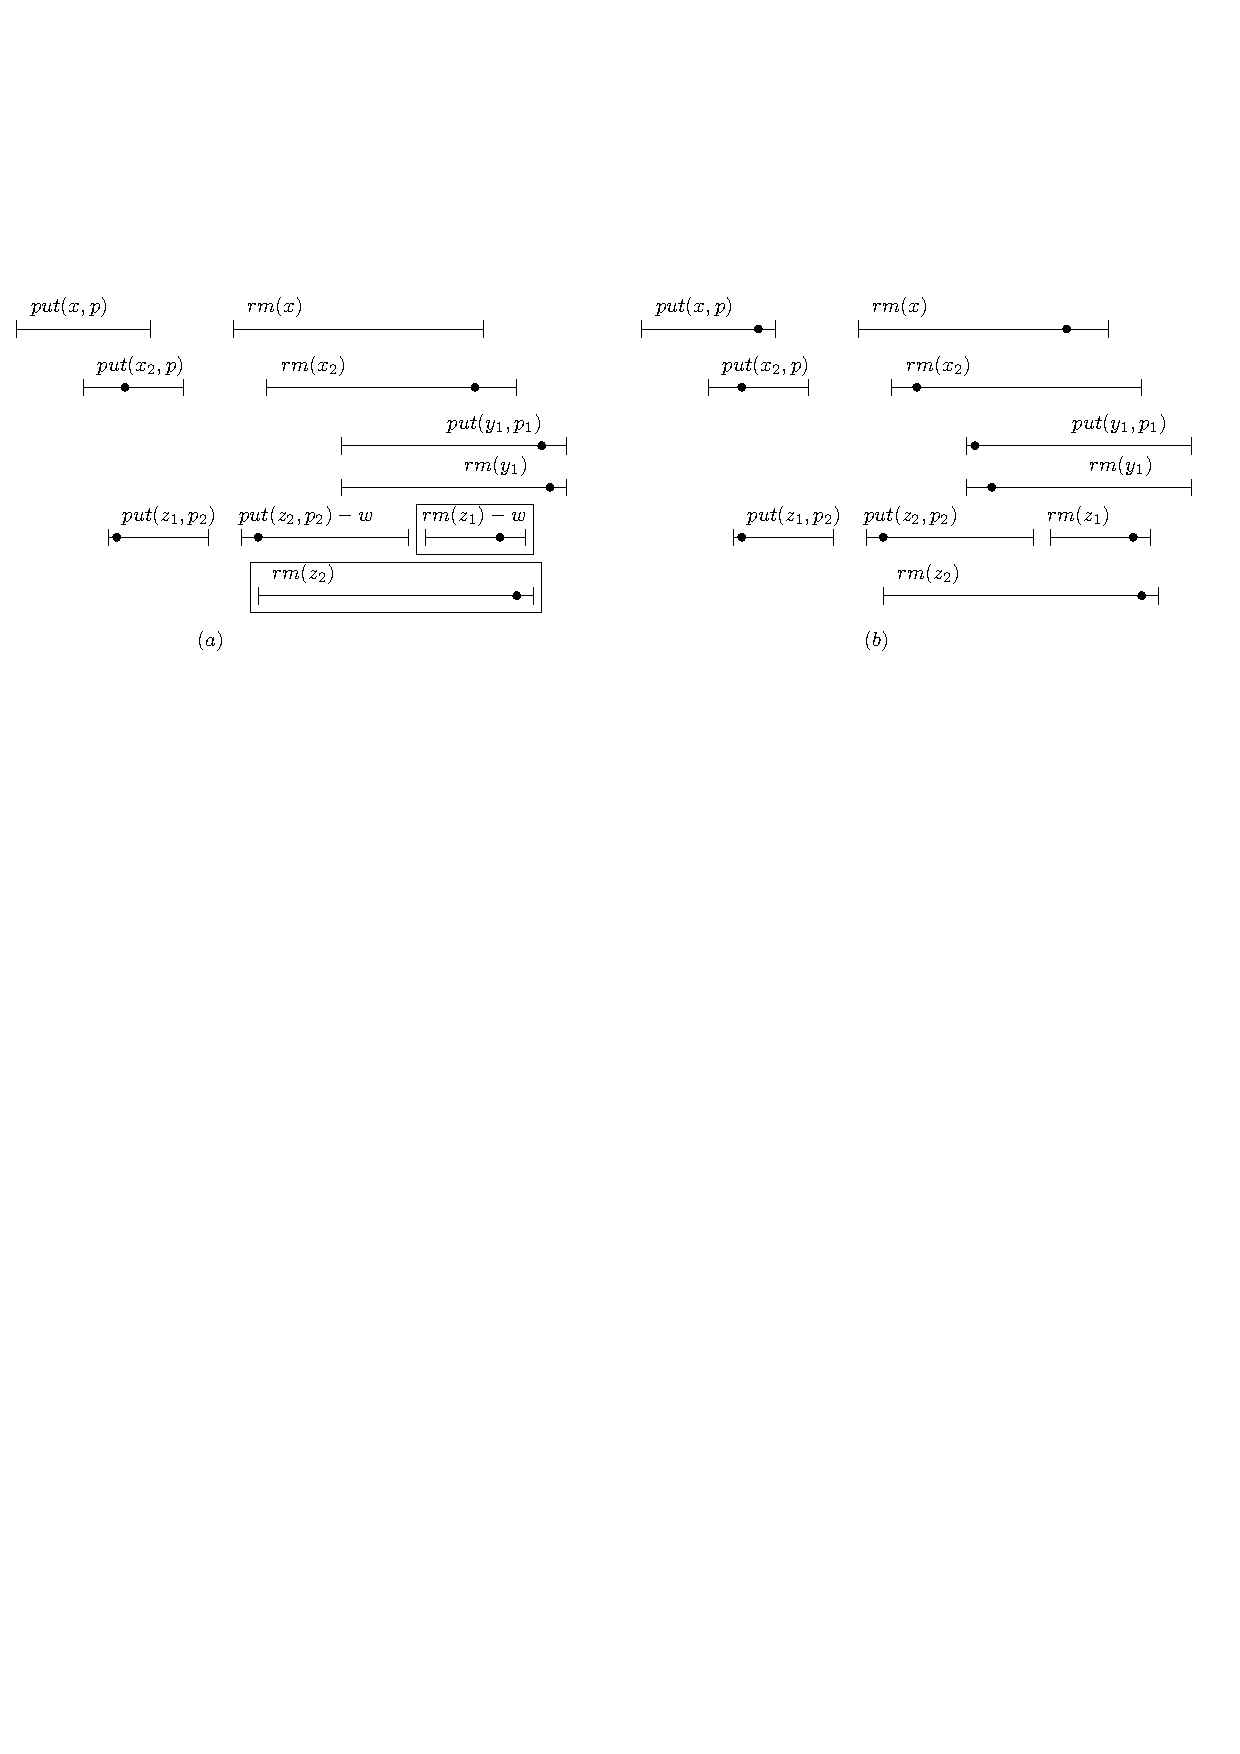
\includegraphics[width=.8\textwidth]{PIC-HIS-EPQ1-TwoHis-2.pdf}
  \caption{A concurrent execution $e$ exemplifying the soundness of $\textit{Check-PQ-Conc}$.}
  \label{fig:concurrent execution for EPQ1}
\end{figure}




Section~\ref{sec:co-regular of extended priority queues} introduces a characterization of concurrent priority queue violations using a set of \emph{non-recursive} automata (whose states consist of a fixed number of registers), whose standard synchronized product is equivalent to $\textit{Check-PQ-Conc}$ (modulo a renaming of values which is possible by data-independence). Since $\seqPQ$ is closed under projection (Lemma~\ref{lem:closure_proj}), the recursion in $\textit{Check-PQ-Conc}$ can be eliminated by checking that each projection of a given execution $e$ passes a non-recursive version of $\textit{Check-PQ-Conc}$ where every recursive call $\text{{\bf return}}\ \textit{Check-PQ-Conc}(\ldots)$ is 
replaced by  $\text{{\bf return}}\ \mathsf{true}$. Let $\textit{Check-PQ-Conc-NonRec}$ be the thus obtained procedure.

\begin{lemma}
\label{lemma:EPQ as multi in MRpri for history}
Given a data-differentiated execution $e$, $e \sqsubseteq \seqPQ$ if and only if for each $e' \in \textit{proj}(e)$, $\textit{Check-PQ-Conc-NonRec}(e')$ returns $\mathsf{true}$.
\end{lemma}








 







\section{Reducing Linearizability of Priority Queues to Reachability}
\label{sec:co-regular of extended priority queues}

We show that the set of executions for which $\textit{Check-PQ-Conc-NonRec}$ fails on some projection can be described using register automata, modulo a value renaming. Renaming values (which is complete under data independence) allows to simplify the reasoning about projections. W.l.o.g., we assume that all the operations which are not in the projection failing this test use the same distinguished value $\top$, different from those in the projection. Then, it is enough to find an automata characterization of the executions $e$ for which $\textit{Check-PQ-Conc-NonRec}(e)$ is $\mathsf{false}$, i.e., for which 
$\Gamma(e) := \mathsf{Has\text{-}}\Gamma(e) \Rightarrow \exists \alpha.\ \Gamma\mathsf{\text{-}Conc}(e,\alpha)$ is false, for some $\Gamma\in \{\mathsf{EmptyRemove}$, $\mathsf{UnmatchedMaxPriority}$, $\mathsf{MatchedMaxPriority}\}$.
Intuitively, $\Gamma(e)$ states that $e$ is linearizable w.r.t. the set of sequential executions described by $\Gamma\mathsf{\text{-}Seq}$ (provided that $\mathsf{Has\text{-}}\Gamma(e)$ holds). Therefore, by an abuse of terminology, an execution $e$ satisfying $\Gamma(e)$ is called \emph{linearizable w.r.t. $\Gamma$}, or \emph{$\Gamma$-linearizable}.
Extending the automaton characterizing non $\Gamma$-linearizable executions with self-loops that allow any operation with argument $\top$ results in an automaton satisfying the following property called \emph{$\Gamma$-completeness}.

\begin{definition}
For $\Gamma\in \{\mathsf{EmptyRemove}$, $\mathsf{UnmatchedMaxPriority}$, $\mathsf{MatchedMaxPriority}\}$, an automaton $A$ is called \emph{$\Gamma$-complete} when for each data-independent implementation $\mathcal{I}$:

$A \cap \mathcal{I} \neq \emptyset$ iff there exists $e \in \mathcal{I}$ and $e' \in \textit{proj}(e)$ such that $e'$ is not $\Gamma$-linearizable.
\end{definition}




We can show that for any $\Gamma\in \{\mathsf{EmptyRemove}$,$\mathsf{UnmatchedMaxPriority}$,$\mathsf{MatchedMaxPriority}\}$ there exists a $\Gamma$-complete automaton. For lack of space, we only consider the case $\Gamma=\mathsf{MatchedMaxPriority}$ in 
Section~\ref{ssec:aut}.
When defining $\Gamma$-complete automata, we assume that every implementation $\mathcal{I}$ behaves correctly, i.e., as a FIFO queue, when only values with the same priority are observed. More precisely, we assume that for every execution $e\in\mathcal{I}$ and every priority $p\in\mathbb{P}$, the projection of $e$ to values with priority $p$ is linearizable (w.r.t. $\seqPQ$). This property can be checked separately using register automata similar to the automata in~\cite{DBLP:conf/icalp/BouajjaniEEH15} describing FIFO queue violations. 
This assumption excludes some obvious violations, such as an $\textit{rm}(a)$ operation happening before a $\textit{put}(a,p)$ operation, for some $p$.

For $\Gamma\in \{\mathsf{UnmatchedMaxPriority}, \mathsf{MatchedMaxPriority}\}$, we consider $\Gamma$-complete automata recognizing executions which contain only one maximal priority. This is w.l.o.g. because any data-differentiated execution for which $\Gamma(e)$ is false has such a projection.
Formally, given a data-differentiated execution $e$ and $p$ a maximal priority in $e$, $e\vert_{\preceq p}$ is the projection of $e$ to the set of values with priorities smaller or equal to $p$. Then,

\begin{lemma}
\label{lemma:pri execution is enough}
For $\Gamma\in \{\mathsf{UnmatchedMaxPriority}, \mathsf{MatchedMaxPriority}\}$, a data-differentiated execution $e$ 
 is $\Gamma$-linearizable iff $e\vert_{\preceq p}$ is $\Gamma$-linearizable for some maximal priority $p$ in $e$.
\end{lemma}
\begin {proof} (Sketch)
For the ``only-if'' direction, let $e$ be a data-differentiated execution linearizable w.r.t. $l = u \cdot \textit{put}(x,p) \cdot v \cdot \textit{rm}(x) \cdot w$ s.t. $\mathsf{MatchedMaxPriority}\mathsf{\text{-}Seq}(l,x)$ holds. Since the predicate $\mathsf{MatchedMaxPriority}\mathsf{\text{-}Seq}(l,x)$ imposes no restriction on the operations in $u$, $v$, and $w$ with priorities incomparable to $p$, erasing all these operations results in a sequential execution which still satisfies this predicate. Similarly, for $\Gamma=\mathsf{UnmatchedMaxPriority}$.

The ``if'' direction follows from the fact that if the projection of an execution to a set of operations $O_1$ has a linearization $l_1$ and the projection of the same execution to the remaining set of operations has a linearization $l_2$, then the execution has a linearization which is defined as an interleaving of $l_1$ and $l_2$. 

Thus, let $e$ be an execution such that $e\vert_{\preceq p}$ is linearizable w.r.t. $l = u \cdot \textit{put}(x,p) \cdot v \cdot \textit{rm}(x) \cdot w$ where $\mathsf{MatchedMaxPriority}\mathsf{\text{-}Seq}(l,x)$ holds. By the property above, we know that $e$ has a linearization $l' = u' \cdot \textit{put}(x,p) \cdot v' \cdot \textit{rm}(x) \cdot w'$, such that the projection of $l'$ to values of priority comparable to $p$ is $l$.
Since $\mathsf{MatchedMaxPriority}\mathsf{\text{-}Seq}(l,x)$ doesn't constrain the values of priority incomparable to $p$, we obtain that $\mathsf{MatchedMaxPriority}\mathsf{\text{-}Seq}(l',\alpha)$ also holds.
\end {proof}

The existence of $\Gamma$-complete automata enable an effective reduction of checking linearizability of concurrent priority queue implementations to state reachability. 
Section~\ref{subsec:combine step-by-step linearizability and co-regular} discusses decidability results implied by this reduction.

\begin{theorem}
\label{lemma:reduce EPQ into state reachability}
Let $\mathcal{I}$ be a data-independent implementation. Then, there is a $\Gamma$-complete automaton $A(\Gamma)$ for each $\Gamma$. Moreover,
$\mathcal{I} \sqsubseteq \seqPQ$ iff $\mathcal{I} \cap A(\Gamma) = \emptyset$ for all $\Gamma$.
\end{theorem}













\subsection{A $\mathsf{MatchedMaxPriority}$-complete automaton}\label{ssec:aut}


A differentiated execution $e$ is not $\mathsf{MatchedMaxPriority}$-linearizable when all the $\textit{put}$ operations in $e$ using the maximal priority $p$ are matched, and $e$ is not linearizable w.r.t. the set of sequential executions satisfying $\mathsf{MatchedMaxPriority\text{-}Seq}(e,x)$ for each value $x$ of priority $p$. We consider two cases depending on whether $e$ contains exactly one value with priority $p$ or at least two values. We denote by $\mathsf{MatchedMaxPriority}^{>}$ the strengthening of $\mathsf{MatchedMaxPriority}$ with the condition that all the values other than $x$ have a priority strictly smaller than $p$ (corresponding to the first case), and by $\mathsf{MatchedMaxPriority}^{=}$ the strengthening of the same formula with the negation of this condition (corresponding to the second case).
We use particular instances of register automata~\cite{DBLP:journals/tcs/KaminskiF94,DBLP:conf/icalp/Cerans94,DBLP:conf/stacs/SegoufinT11} whose states include only two registers, one for storing a priority guessed at the initial state, and one for storing the priority of the current action in the execution. The transitions can check equality or the order relation $\prec$ between the values stored in the two registers. Instead of formalizing the full class of register automata, we consider a simpler class which suffices our needs. Thus, we consider a class of labeled transition systems whose states consist of a finite control part and a register $r$ interpreted to elements of $\mathbb{P}$. The transition labels are:
\begin{itemize}
	\item $r=*$ for storing an arbitrary value to $r$,
	\item $\textit{call}(\textit{rm},a)$ and $\textit{ret}(\textit{rm},a)$ for reading call/return actions of a remove,
	\item $\textit{call}(\textit{put},d,g)$ where $g\in\{=r,\prec r,true\}$ is a guard, for reading a call action $\textit{call}(\textit{put},d,p)$ and checking if $p$ is either equal to or smaller than the value stored in $r$, or arbitrary,
	\item $\textit{ret}(\textit{put},d,true)$ for reading a return action $\textit{ret}(\textit{put},d,p)$ for any $p$.
\end{itemize}
The set of sequences (executions) accepted by such a transition system is defined as usual.



\subsubsection{A $\mathsf{MatchedMaxPriority}^>$-complete automaton}
\label{subsec:co-regular of EPQ1Lar}

\begin{figure}[t]
  \centering
  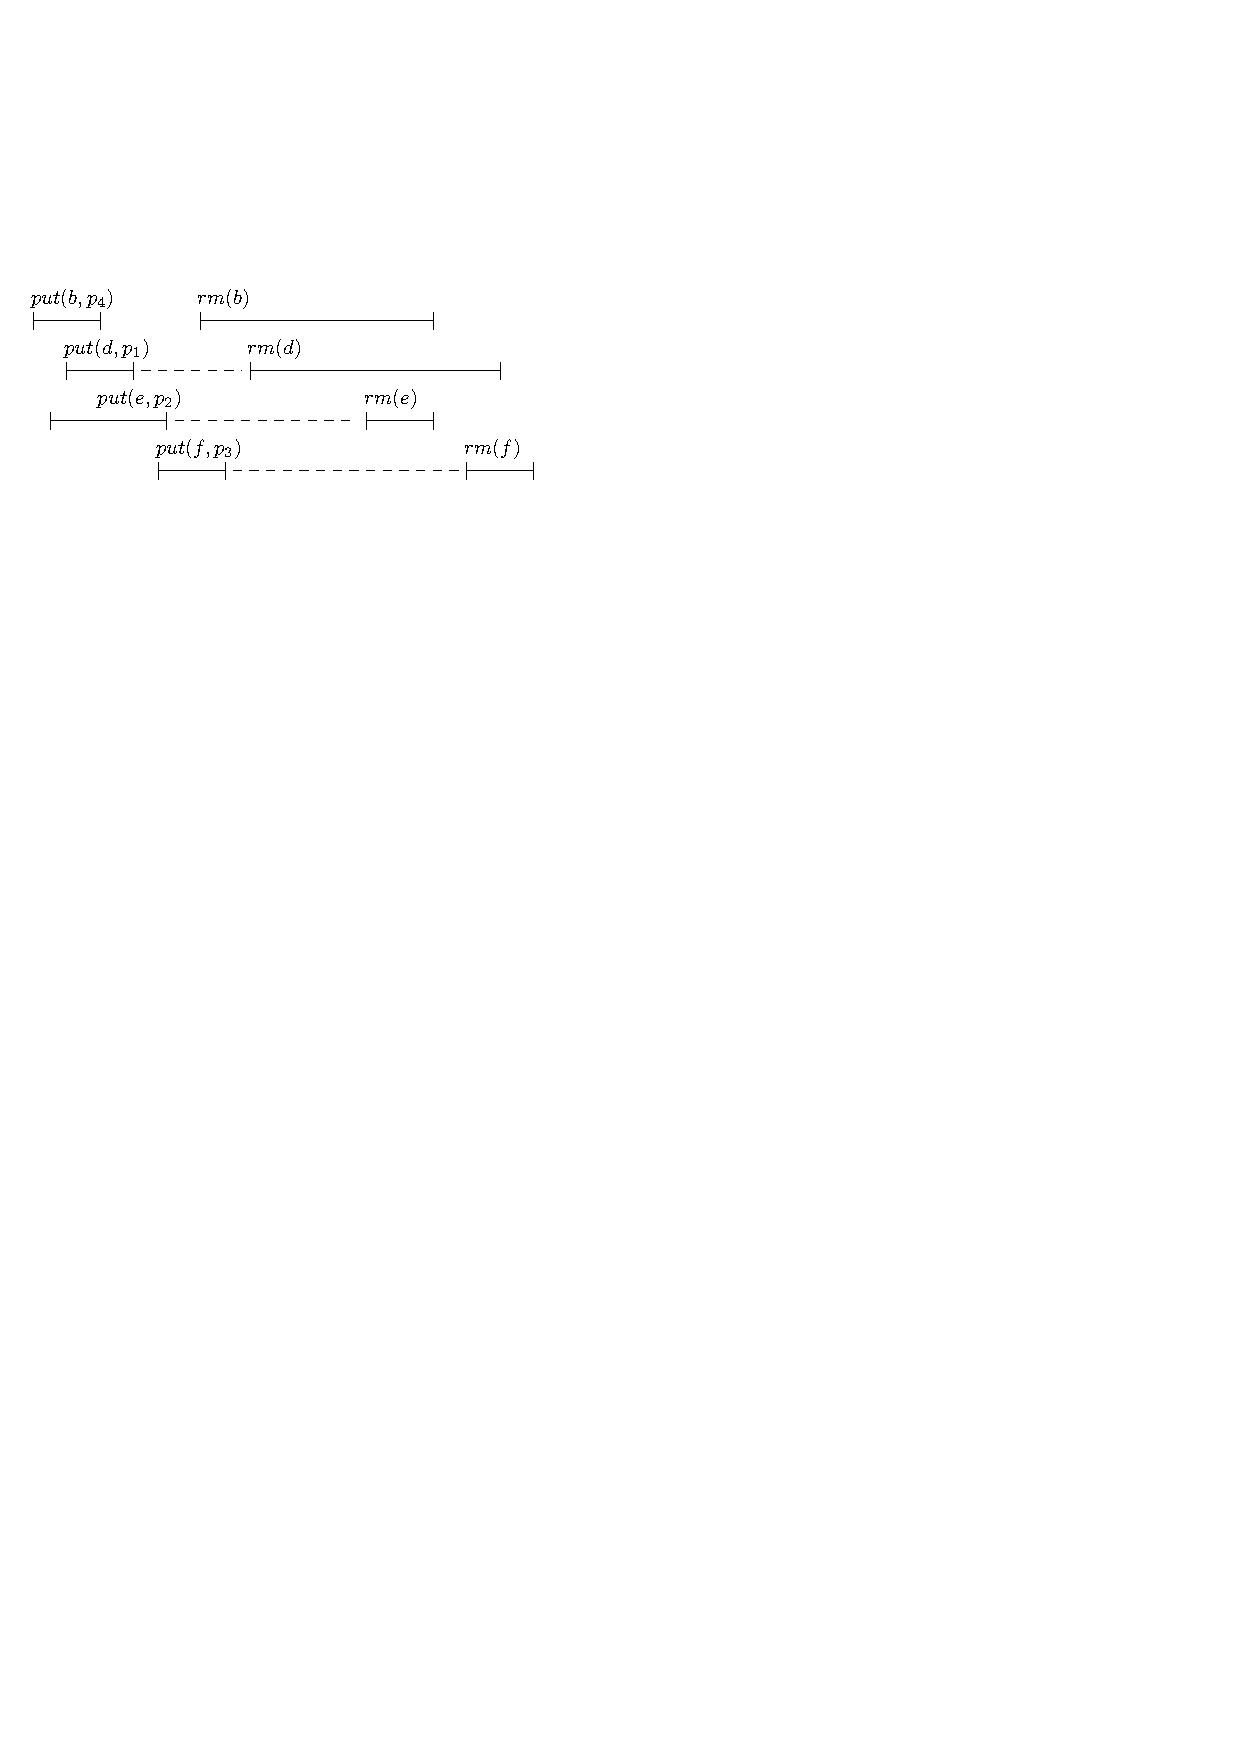
\includegraphics[width=0.4 \textwidth]{PIC-HIS-INTRO-GAP-EPQ1L.pdf}
  \caption{An execution that is not $\mathsf{MatchedMaxPriority}^{>}$-linearizable. We represent each operation as a time interval whose left, resp., right, bound corresponds to the call, resp., return action.} 
  \label{fig:introduce gap for EPQ1Lar}
\end{figure}






Figure~\ref{fig:introduce gap for EPQ1Lar} contains a typical example of an execution $e$ which is not $\mathsf{MatchedMaxPriority}^>$-linearizable,
where $p_1 \prec p_4$, $p_2 \prec p_4$, and $p_3 \prec p_4$.
Intuitively, this is a violation because during the whole execution of $\textit{rm}(b)$, the priority queue stores a smaller priority value (which should be removed before $b$). To be more precise, we define \emph{the interval of a value $x$} as the time interval from the return of a put $\textit{ret}(\textit{put},x,p)$ to the call of the matching remove $\textit{call}(rm,x)$, or to the end of the execution if such a call action doesn't exist. This represents the time interval in which a value is guaranteed to be stored into the priority queue. Concretely, for a standard indexing of actions in an execution, a time interval is a closed interval between the indexes of two actions in the execution.
In \figurename~\ref{fig:introduce gap for EPQ1Lar}, the interval of each value of priority smaller than $p_4$ is pictured as a dashed line. There is no sequence $l$ s.t. $e \sqsubseteq l$ and $\mathsf{MatchedMaxPriority}\mathsf{\text{-}Seq}(l,b)$ hold, since each time point from $\textit{call}(\textit{rm},b)$ to $\textit{ret}(\textit{rm},b)$ is included in the interval of a smaller priority value, 
and $\textit{rm}(b)$ can't take effect in the interval of a smaller priority value.
To formalize this scenario we use the notion of \emph{left-right constraint} defined below.



\begin{definition}\label{def:left-right constraint for matched put and rm operations}
Let $e$ be a data-differentiated execution which contains only one maximal priority $p$, and only one value $x$ of priority $p$ (and no $\textit{rm}(\textit{empty})$ operations).
The \emph{left-right constraint of $x$} is the graph $G$ where: 
\begin{itemize}
\item the nodes are the values occurring in $e$, 
\item there is an edge from $d_1$ to $x$, if $\textit{put}(d_1,\_) <_{\textit{hb}} \textit{put}(x,p)$ or $\textit{put}(d_1,\_) <_{\textit{hb}} \textit{rm}(x)$,
\item there is an edge from $x$ to $d_1$, if $\textit{rm}(x)<_{\textit{hb}}\textit{rm}(d_1)$ or $\textit{rm}(d_1)$ does not exists,
\item there is an edge from $d_1$ to $d_2$, if $\textit{put}(d_1,\_) <_{\textit{hb}} \textit{rm}(d_2,\_)$.
\end{itemize}
\end{definition}

The execution in \figurename~\ref{fig:introduce gap for EPQ1Lar} is not $\mathsf{MatchedMaxPriority}^>$-linearizable because the left-right constraint of the maximal priority value $b$ contains the cycle $f \rightarrow d \rightarrow c \rightarrow b \rightarrow f$. The presence of such a cycle is equivalent to \emph{non} $\mathsf{MatchedMaxPriority}^>$-linearizability:

\begin{lemma}
\label{lemma:Lin Equals Constraint for EPQ1Lar}
Let $e$ be a data-differentiated execution such that 
$\mathsf{Has\text{-}MatchedMaxPriority}(e)$ holds, $p$ is the maximal priority in $e$, and $\textit{put}(x,p)$ and $\textit{rm}(x)$ are only operations with arguments of priority $p$ in $e$. 
Then, $e$ is $\mathsf{MatchedMaxPriority}$-linearizable iff the left-right constraint of $x$ contains no cycle going through $x$.
\end{lemma}

When the left-right constraint contains a cycle $d_1 \rightarrow \ldots \rightarrow d_m \rightarrow x \rightarrow d_1$, for some $d_1$,$\ldots$,$d_n\in \mathbb{D}$, we say that $x$ is \emph{covered} by $d_1,\ldots,d_m$. The shape of an execution witnessing such a cycle (i.e., the alternation between call/return actions) can be identified using our class of automata, the only complication being the unbounded number of values $d_1$,$\ldots$,$d_n$. However, by data independence, whenever an implementation contains such an execution it also contains an execution where all the values $d_1$,$\ldots$,$d_n$ are renamed to the same value $a$, and $x$ is renamed to $b$. Therefore, our automata can be defined over a fixed set of values $a$, $b$, and $\top$ (recall that $\top$ is used for operations outside of the non-linearizable projection).

To define a $\mathsf{MatchedMaxPriority}^>$-complete automaton, we need to consider all the possible orders between the call/return actions of the $\textit{put}$/$\textit{rm}$ operations that add and respectively, remove the value $b$. The case where the put happens-before the remove (as in \figurename~\ref{fig:introduce gap for EPQ1Lar}) is pictured in \figurename~\ref{fig:automata APQ1Lar-1 in paper}. This automaton captures the three possible ways of ordering the first action $\textit{ret}(\textit{put},a,\_)$ w.r.t. the actions with value $b$, which are pictured in \figurename~\ref{fig:executions APQ1Lar-1 in paper}(a) (this action cannot occur after $\textit{call}(\textit{rm},b,\_)$ since $b$ must be covered by the $a$-s). The paths corresponding to these three possible orders are: $q_1 \rightarrow q_2 \rightarrow q_3 \ldots \rightarrow q_7$, $q_1 \rightarrow q_2 \rightarrow q_3 \ldots \rightarrow q_{10}$, and $q_1 \rightarrow q_9 \rightarrow q_{10} \ldots \rightarrow q_7$. \figurename~\ref{fig:executions APQ1Lar-1 in paper} lists the four possible orderings of the call/return actions of adding and removing $b$, and also possible orders of the first $\textit{ret}(\textit{put},a,\_)$ w.r.t the actions with value $b$. Each such ordering corresponds to an automaton similar to the one in \figurename~\ref{fig:automata APQ1Lar-1 in paper}, their union defining a $\mathsf{MatchedMaxPriority}^>$-complete automaton.




\begin{figure}[t]
  \centering
  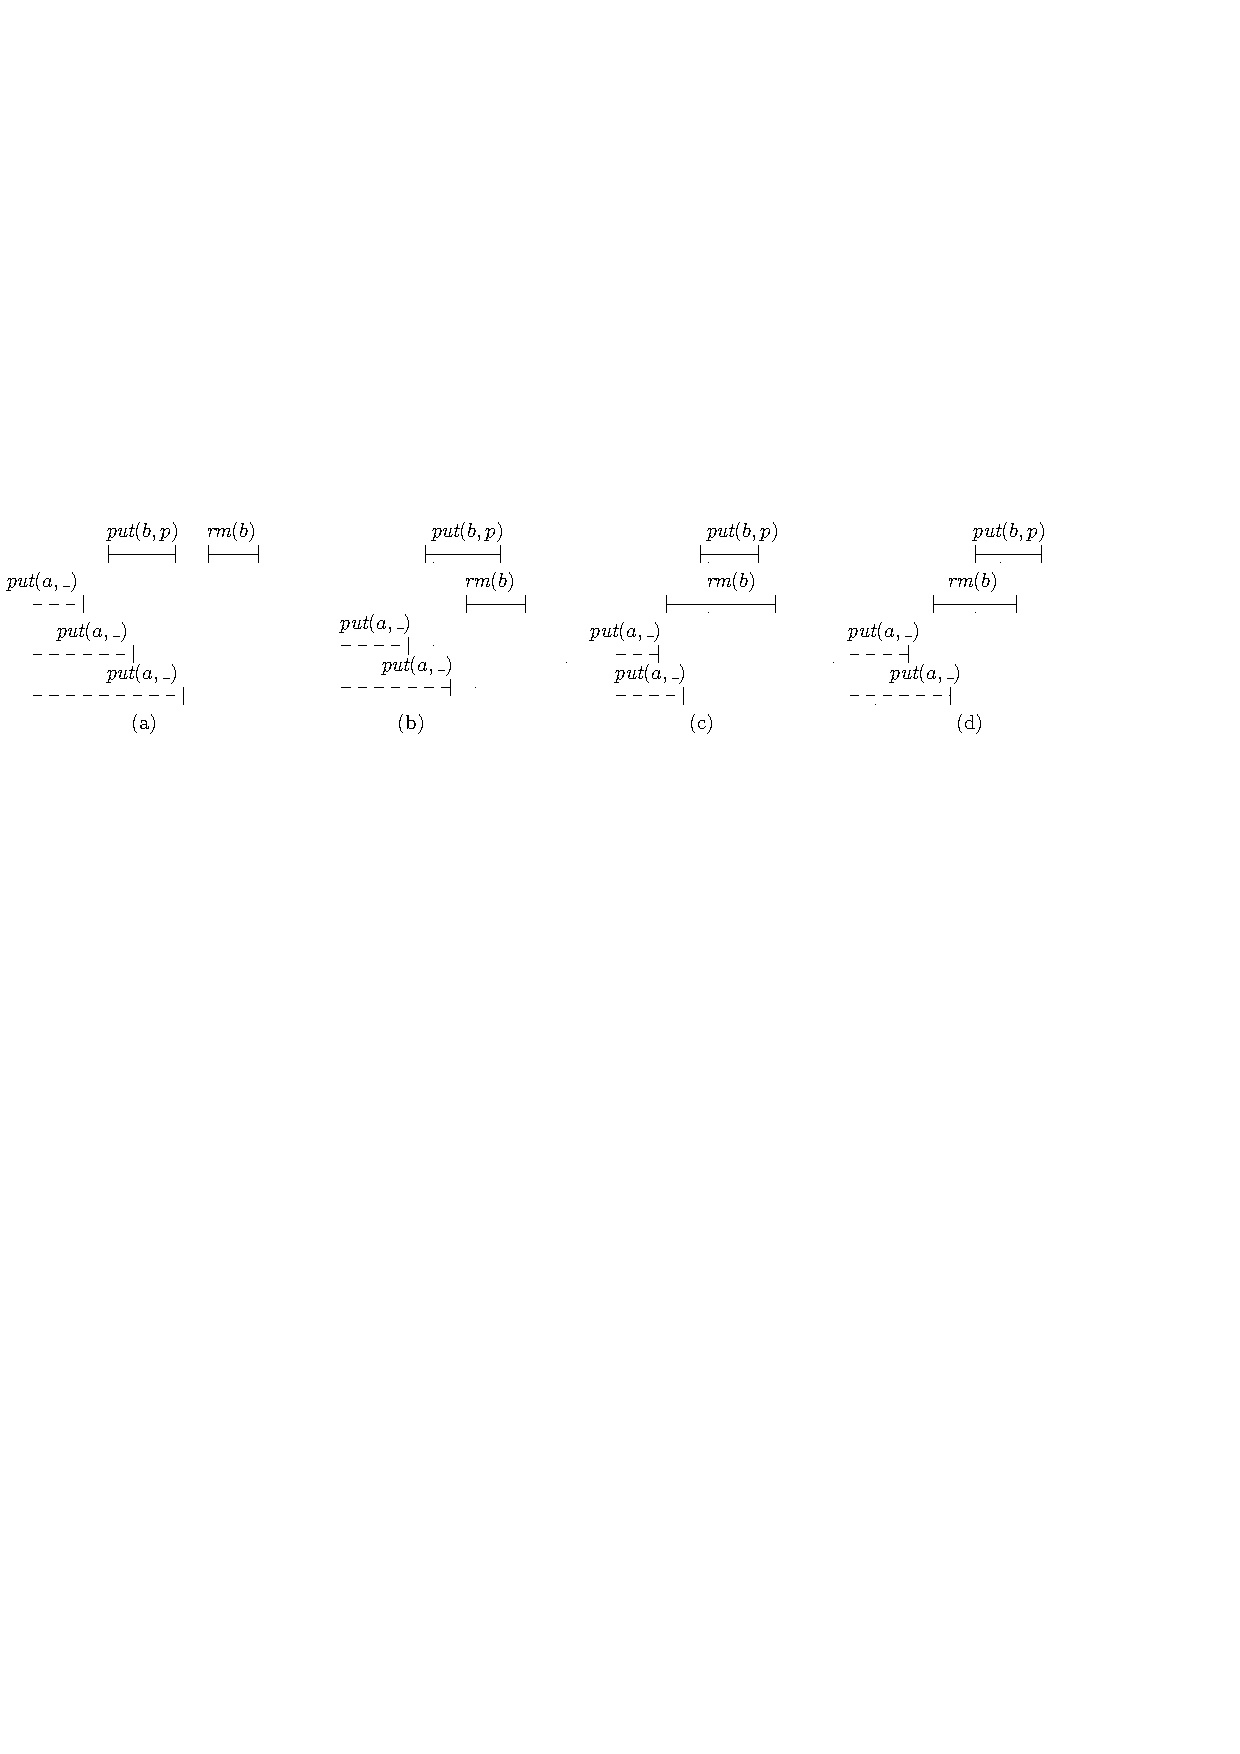
\includegraphics[width=.8\textwidth]{PIC_HIS_PQ1Lar-fouCase.pdf}
  \caption{Orderings to be considered when defining a $\mathsf{MatchedMaxPriority}^>$-complete automaton.}
  \label{fig:executions APQ1Lar-1 in paper}
\end{figure}

\begin{figure}[t]
  \centering
  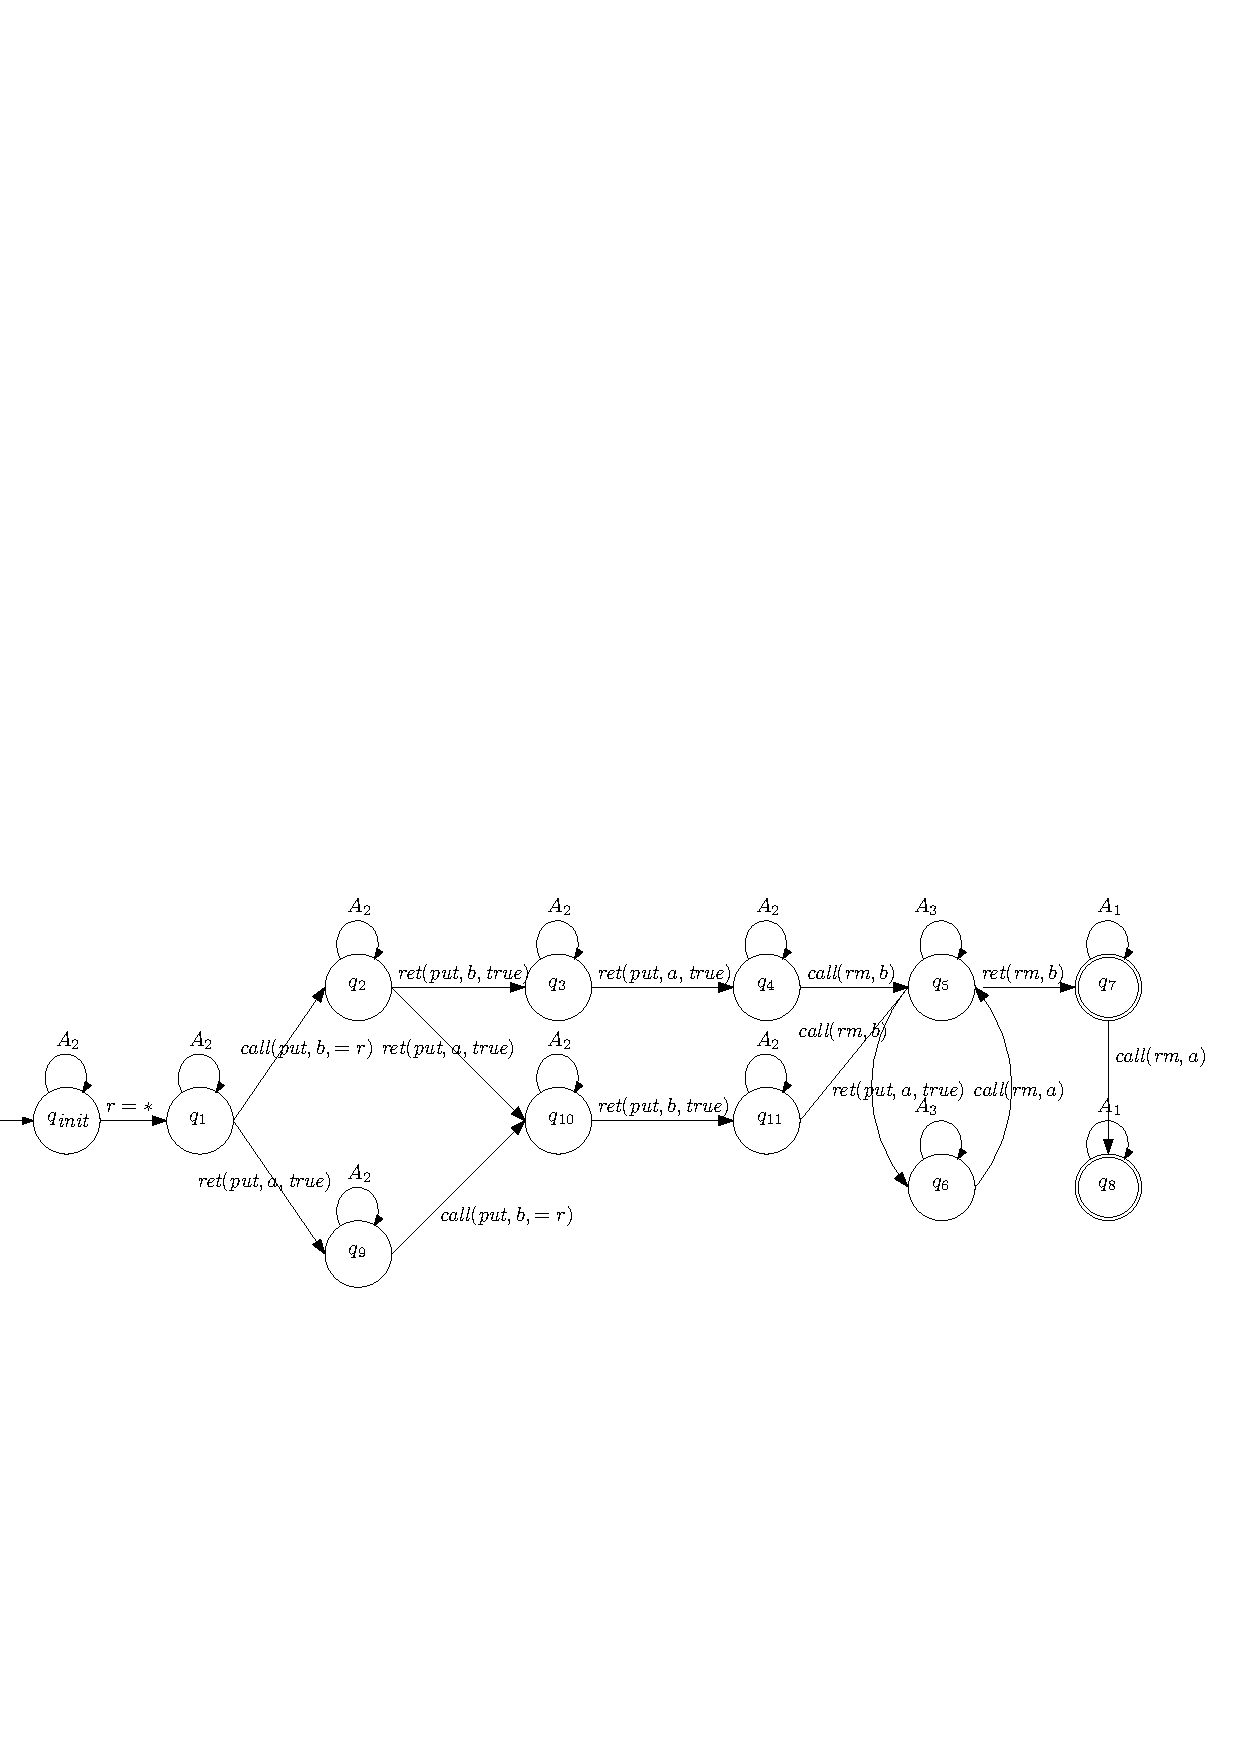
\includegraphics[width=.9\textwidth]{PIC_AUTO_PQ1Lar-pprr.pdf}
  \caption{A register automaton capturing the scenario in Figure~\ref{fig:executions APQ1Lar-1 in paper}(a). We use the following notations: $A_1 = A \cup \{ \textit{ret}(\textit{rm},a) \}$, $A_2 = A \cup \{ \textit{call}(\textit{put},a,=r) \}$, $A_3 = A_2 \cup \{ \textit{ret}(\textit{rm},a) \}$, where $A = \{ \textit{call}(\textit{put},\top,\textit{true}),\textit{ret}(\textit{put},\top,\textit{true}), \textit{call}(\textit{rm},\top)$, $\textit{ret}(\textit{rm},\top),\textit{call}(\textit{rm},\textit{empty}),\textit{ret}(\textit{rm},\textit{empty}) \}$.}
  \label{fig:automata APQ1Lar-1 in paper}
\end{figure}







\subsubsection{A $\mathsf{MatchedMaxPriority}^=$-complete automaton}
\label{subsec:co-regular of EPQ1Equal}

When an execution contains at least two values of maximal priority, the acyclicity of the left-right constraints (for all the maximal priority values) is not enough to conclude that the execution is $\mathsf{MatchedMaxPriority}$-linearizable.
Intuitively, there may exist a value $a$ which is added before another value $b$ such that all the possible linearization points of $\textit{rm}(b)$ are disabled by the position of $\textit{rm}(a)$ in the happens-before. We give an example of such an execution $e$ in \figurename~\ref{fig:introduce pb order}, where $p_1\prec p_4$. This execution  is not linearizable w.r.t. $\mathsf{MatchedMaxPriority}$ (or $\mathsf{MatchedMaxPriority}^{=}$) even if
neither $a$ nor $b$ are covered by values with smaller priority. 
Since $\textit{put}(a,p_4) <_{\textit{hb}} \textit{put}(b,p_4)$ and values of the same priority are removed in FIFO order, $\textit{rm}(a)$ should be linearized before $\textit{rm}(b)$ (i.e., this execution should be linearizable w.r.t. a sequence where $\textit{rm}(a)$ occurs before $\textit{rm}(b)$).
Since $\textit{rm}(b)$ cannot take effect during the interval of a smaller priority value, it could be only linearized in one of the two time intervals pictured with dotted lines in \figurename~\ref{fig:introduce pb order}. However, each of those time intervals ends before $\textit{call}(\textit{rm},a)$, and thus $\textit{rm}(a)$ cannot be linearized before $\textit{rm}(b)$.

\begin{figure}[t]
  \centering
  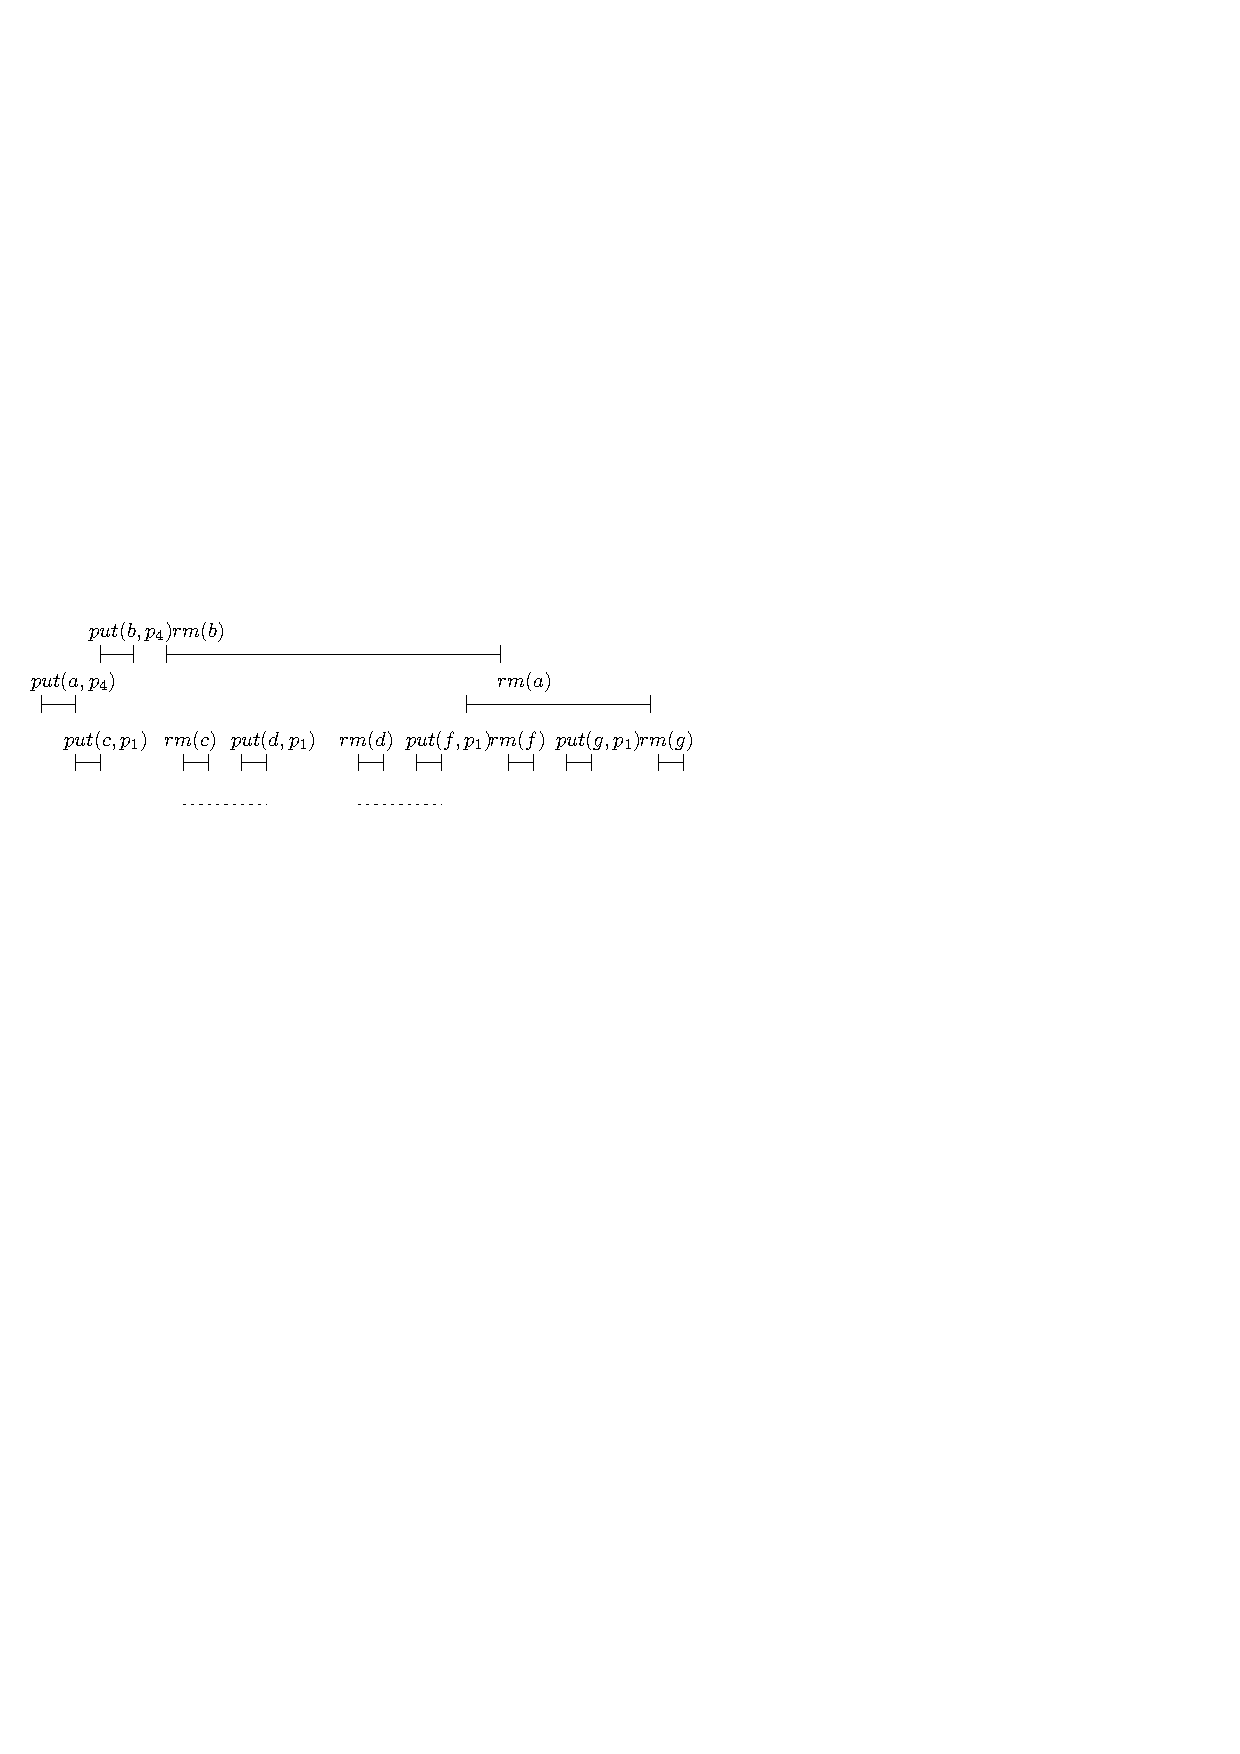
\includegraphics[width=0.5 \textwidth]{PIC-HIS-INTRO-PB-ORDER-EPQ.pdf}
  \caption{An execution that is not $\mathsf{MatchedMaxPriority}^=$-linearizable.}
  \label{fig:introduce pb order}
\end{figure}

To recognize the scenarios in \figurename~\ref{fig:introduce pb order}, we introduce an order $<_{\textit{pb}}$ between values which intuitively, can be thought of as ``a value $a$ is put before another value $b$''. 
More precisely, given a data-differentiated execution $e$ and two values $a$ and $b$ of maximal priority, $a <_{\textit{pb}} b$ if one of the following holds: (1) $\textit{put}(a,\_) <_{\textit{hb}} \textit{put}(b,\_)$, (2) $\textit{rm}(a) <_{\textit{hb}} \textit{rm}(b)$, or (3) $\textit{rm}(a) <_{\textit{hb}} \textit{put}(b,\_)$. Sometimes we use $a <_{\textit{pb}}^A b$, $a <_{\textit{pb}}^B b$, and $a <_{\textit{pb}}^C b$ to explicitly distinguish between these three cases. Let $<_{\textit{pb}}^*$ be the transitive closure of $<_{\textit{pb}}$.

To define the time intervals in which a remove like $\textit{rm}(b)$ in \figurename~\ref{fig:introduce pb order}, can be linearized (outside of intervals of smaller priority values) we use the notion of gap-point. As before, defining time intervals relies on an indexing of actions in an execution, starting with 0.

\begin{definition}\label{def:gap-point for matched put and rm operations}
Let $e$ be a data-differentiated execution with only one maximal priority $p$, and $\textit{put}(x,p)$ and $\textit{rm}(x)$ two operations in $e$. An index $i\in [0,|e|-1]$ is a \emph{gap-point of $x$} if $i$ is greater than or equal to the index of both $\textit{call}(\textit{put},x,p)$ and $\textit{call}(\textit{rm},x)$, smaller than the index of $\textit{ret}(\textit{rm},x)$, and not included in the interval of a value with priority smaller than $p$.
\end{definition}

The case of \figurename~\ref{fig:introduce pb order} can be formally described as follows: $a <_{\textit{pb}}^* b$ while the right-most gap-point of $b$ is before $\textit{call}(\textit{rm},a)$ or $\textit{call}(\textit{put},a,p_4)$. The following lemma states that these conditions are enough to characterize non-linearizability w.r.t. $\mathsf{MatchedMaxPriority}^{=}$. 

\begin{lemma}
\label{lemma:EPQ1Equal as pb order and gap-point}
Let $e$ be a data-differentiated execution with only one maximal priority $p$ such that $\mathsf{Has\text{-}MatchedMaxPriority}(e)$ holds.
Then, $e$ is not $\mathsf{MatchedMaxPriority}^{=}$-linearizable iff $e$ contains two values $x$ and $y$ of maximal priority $p$ such that $y <_{\textit{pb}}^* x$, and the rightmost gap-point of $x$ is strictly smaller than the index of $\textit{call}(\textit{put},y,p)$ or $\textit{call}(\textit{rm},y)$.
\end{lemma}


The following shows that the number of values needed to witness that $y <_{\textit{pb}}^* x$, for some $x$ and $y$, is bounded.

\begin{lemma}
\label{lemma:ob order has bounded length}
Let $e$ be a data-differentiated execution such that $a <_{\textit{pb}} a_1 <_{\textit{pb}} \ldots <_{\textit{pb}} a_m <_{\textit{pb}} b$ holds for some set of values $a$, $a_1$,$\ldots$,$a_m$, $b$. Then, one of the following holds:
\begin{itemize}
\item[-] $a <_{\textit{pb}}^A b$, $a <_{\textit{pb}}^B b$, or $a <_{\textit{pb}}^C b$,

\item[-] $a <_{\textit{pb}}^A a_i <_{\textit{pb}}^B b$ or $a <_{\textit{pb}}^B a_i <_{\textit{pb}}^A b$, for some $i$.
\end{itemize}
\end{lemma}

\begin{figure}[t]
  \centering
  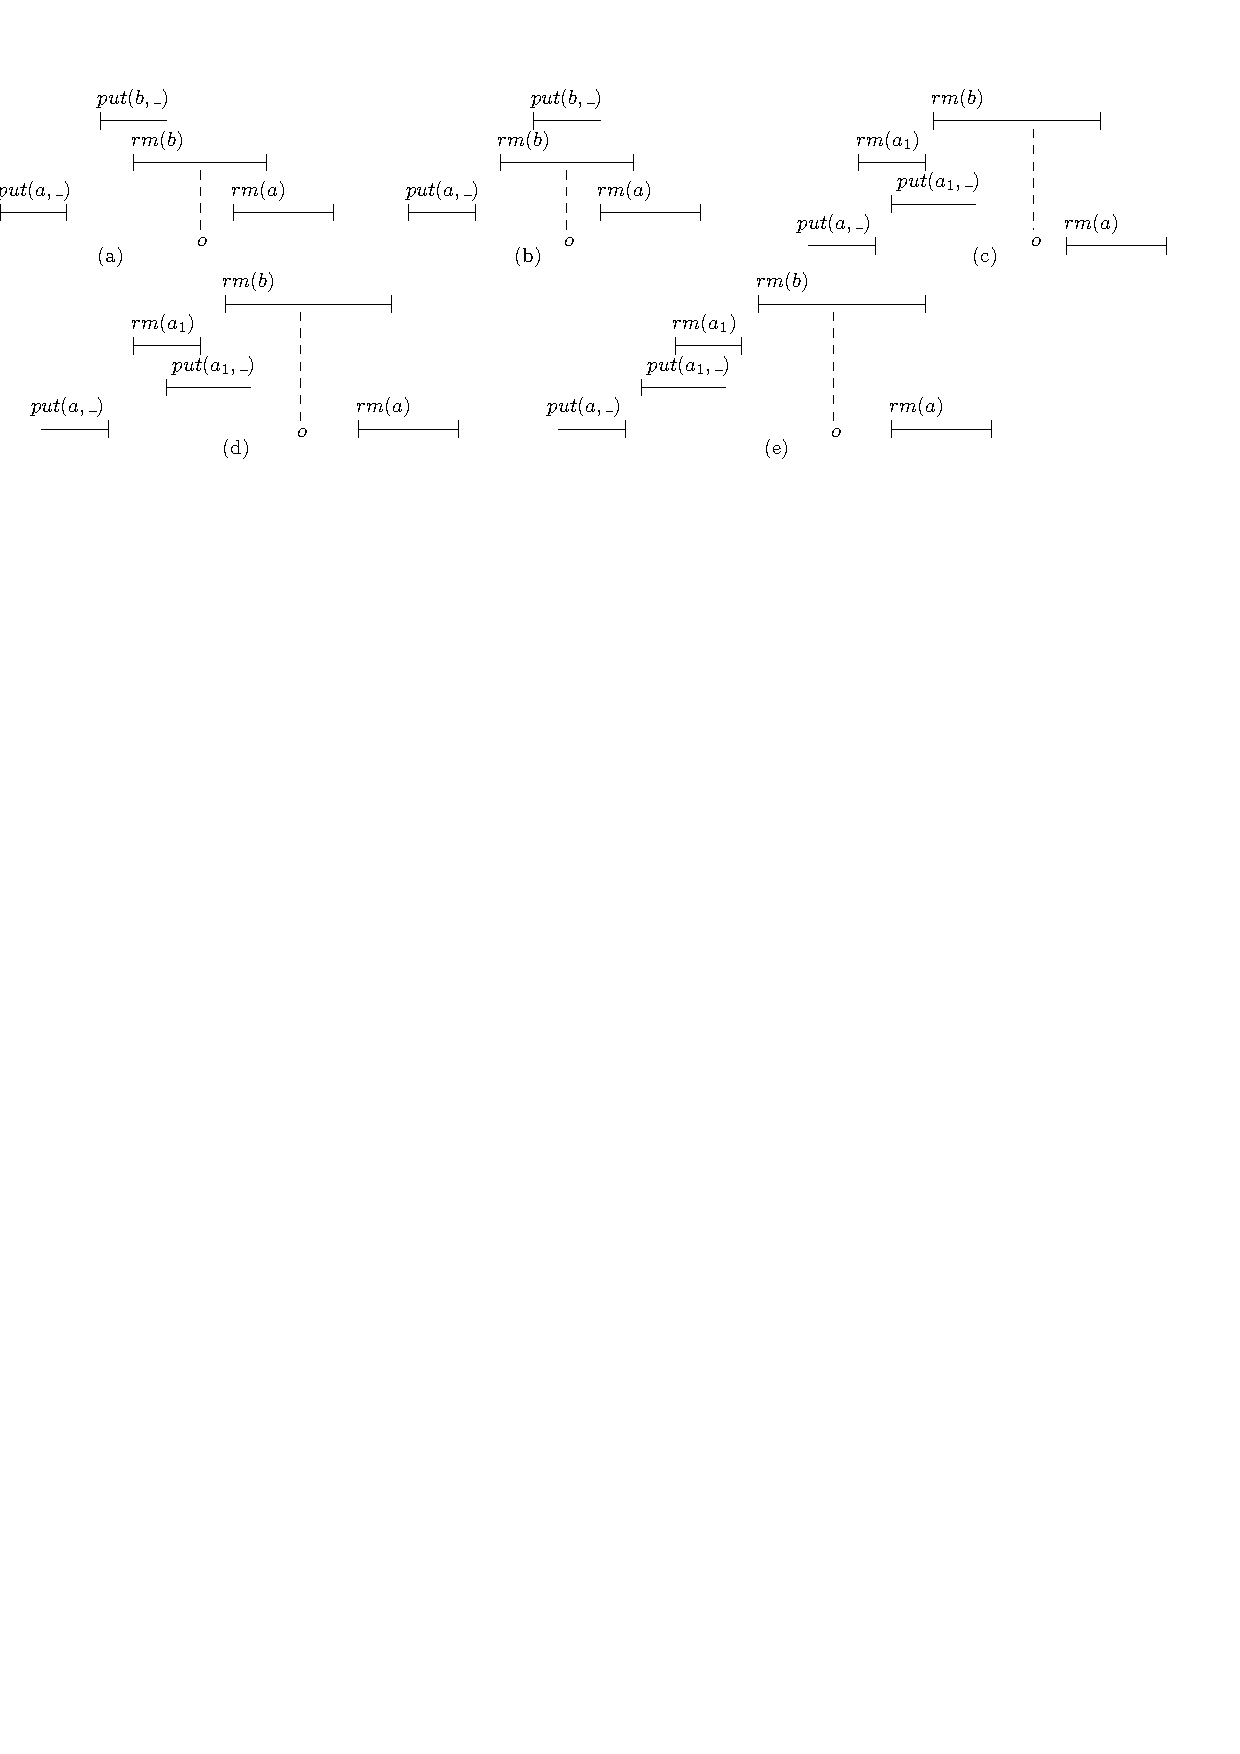
\includegraphics[width=0.8 \textwidth]{PIC-HIS-FiveEnumerations.pdf}
  \caption{Orderings to be considered when defining a $\mathsf{MatchedMaxPriority}^=$-complete automaton. We omit the operations which can be ordered arbitrarily, e.g., $\textit{put}(b)$ in the cases (d) and (e).}
  \label{fig:five enumerations}
\end{figure}

To characterize violations to $\mathsf{MatchedMaxPriority}^{=}$-linearizability, one has to consider all the possible orders between call/return actions of the operations on values $a$, $b$, and $a_i$ in Lemma \ref{lemma:ob order has bounded length}, and the right-most gap point of $b$. Excluding the inconsistent cases, we are left with the five orders in \figurename~\ref{fig:five enumerations}, where $o$ denotes the rightmost gap-point of $b$.
For each case, we define an automaton recognizing the induced set of violations. The register automaton for the case in \figurename~\ref{fig:five enumerations}(a) is shown in \figurename~\ref{fig:an enumeration and its witness automaton}. In this case, Lemma~\ref{lemma:EPQ1Equal as pb order and gap-point} is equivalent to the fact that intuitively, the time interval from $\textit{call}(\textit{rm},a)$ to $\textit{ret}(\textit{rm},b)$ is covered by lower priority values (thus, there is no gap-point of $b$ which occurs after $\textit{call}(\textit{rm},a)$). By data-independence, these lower priority values can be renamed to a fixed value $c$. 









\begin{figure}[t]
  \centering
  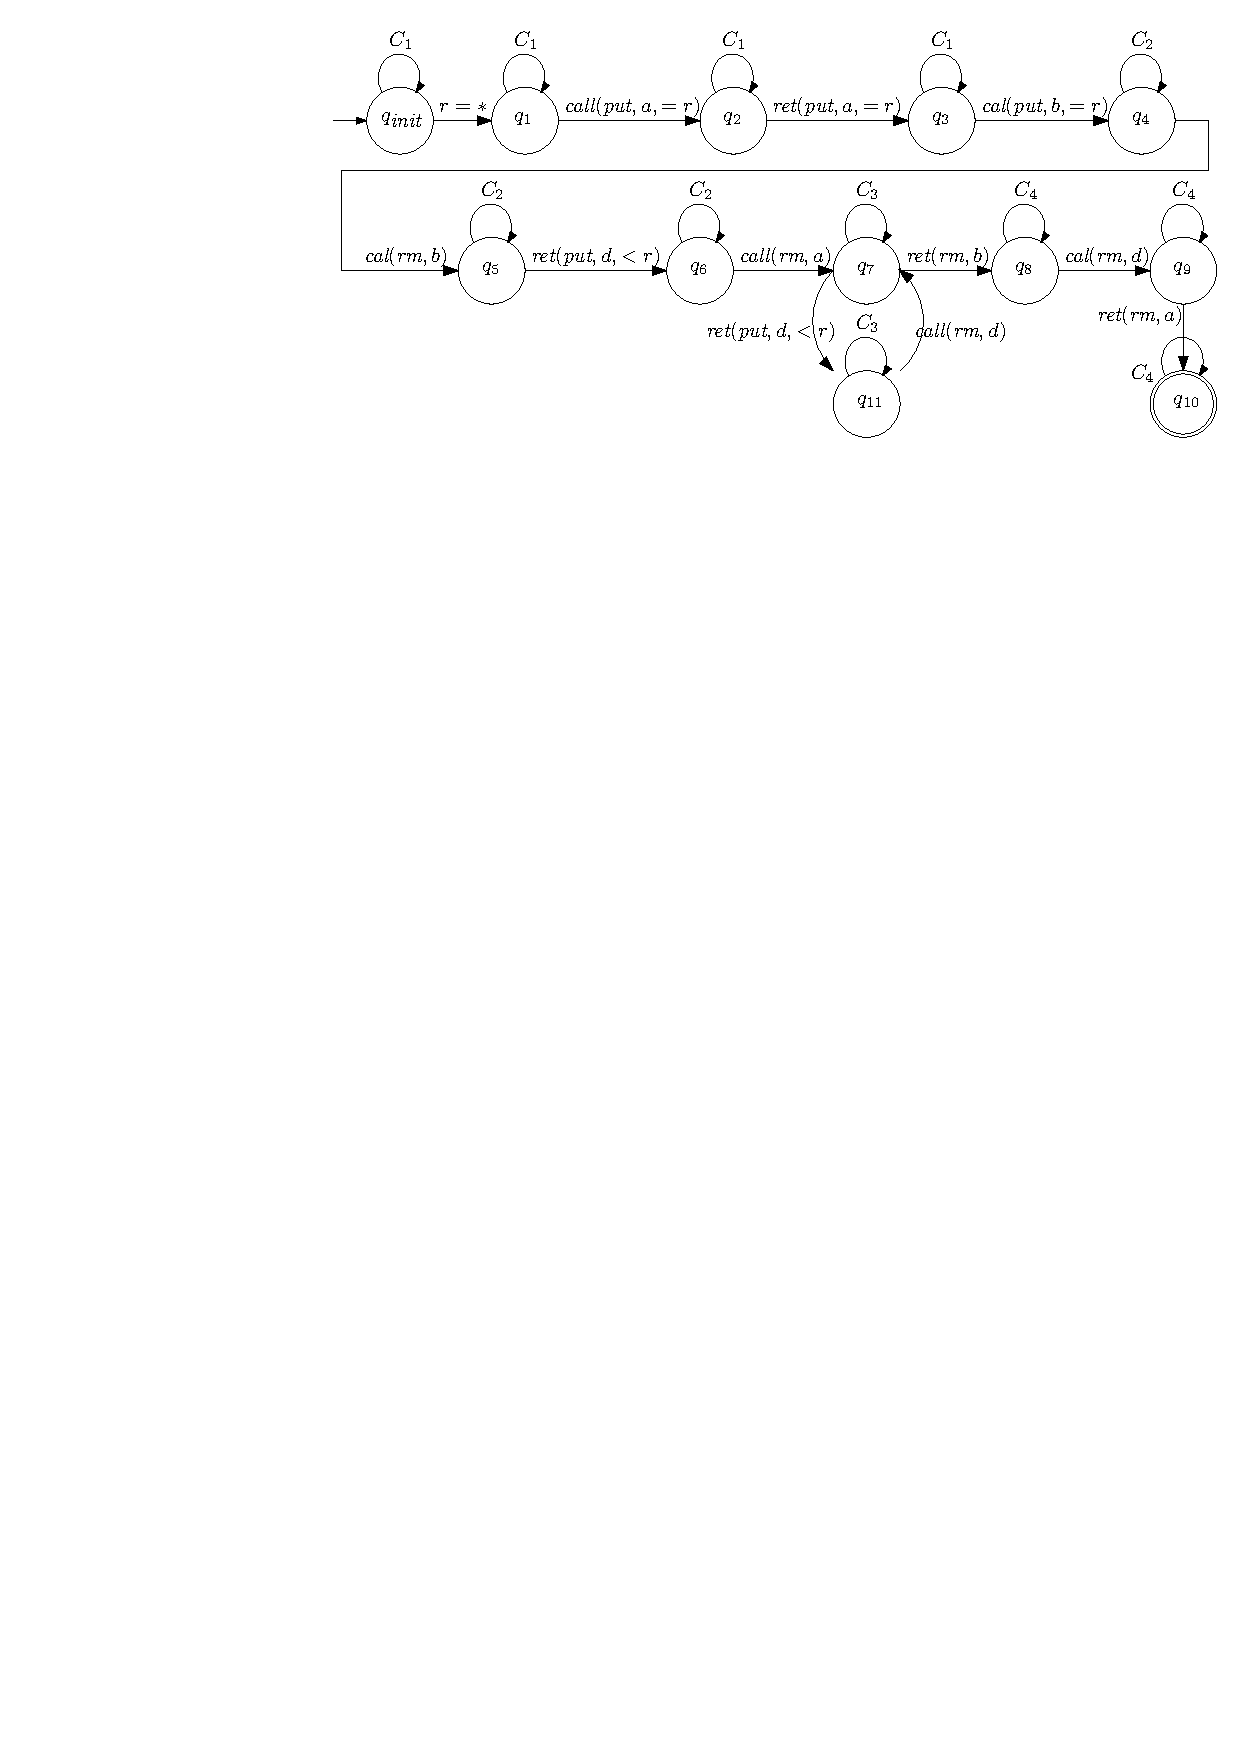
\includegraphics[width=0.65 \textwidth]{PIC-WitnessAutomata-For1.pdf}
  \caption{A register automaton for the case in Figure~\ref{fig:five enumerations}(a), where $A_1 = A \cup \{ \textit{call}(\textit{put},c,<r)\}$, $A_2 = A_1 \cup \{ \textit{ret}(\textit{put},b,=r) \}$, $A_3 = A_2 \cup \{ \textit{ret}(\textit{rm},c) \}$, $A_4 = A \cup \{ \textit{ret}(\textit{put},b,=r), \textit{ret}(\textit{rm},c) \}$, where $A = \{ \textit{call}(\textit{put},\top,\textit{true})$,$\textit{ret}(\textit{put},\top,\textit{true})$,$\textit{call}(\textit{rm},\top)$,$\textit{ret}(\textit{rm},\top)$,$\textit{call}(\textit{rm},\textit{empty})$,$\textit{ret}(\textit{rm},\textit{empty})\}$.}
  \label{fig:an enumeration and its witness automaton}
\end{figure}






\subsection{Decidability Result}
\label{subsec:combine step-by-step linearizability and co-regular}

We describe a class $\mathcal{C}$ of data-independent implementations for which linearizability w.r.t. $\seqPQ$ is decidable. The implementations in $\mathcal{C}$ allow an unbounded number of values but a bounded number of priorities. Each method has a finite set of local variables storing Boolean values or values from $\mathbb{D}$. Methods communicate through a finite number of shared variables interpreted also as Booleans or values from $\mathbb{D}$. To ensure data independence, values in $\mathbb{D}$ may be assigned, but never used in Boolean expressions (e.g., of if-then-else statements). This class captures typical implementations, or finite-state abstractions thereof, e.g., obtained via predicate abstraction. The $\Gamma$-complete automata we define use a fixed set $D=\{a,b,c,a_1,\top\}$ of values ($a_1$ is needed to deal with the second item in Lemma~\ref{lemma:ob order has bounded length}). Therefore, for any $\Gamma$, $\mathcal{C}\cap A(\Gamma)\neq\emptyset$ iff $\mathcal{C}_D\cap A(\Gamma)\neq\emptyset$, where $\mathcal{C}_D$ is the subset of $\mathcal{C}$ that uses only values in $D$. 

The set of executions $\mathcal{C}_D$ can be represented by a Vector Addition System with States (VASS). Since the set of values and priorities is bounded, each method invocation can be represented by a finite-state automaton (see~\cite{conf/esop/BouajjaniEEH13}). For a fixed set of priorities $P\subseteq \mathbb{P}$, the register automata $A(\Gamma)$ can be transformed to finite-state automata (the number of valuations of the registers is bounded). Thus, checking linearizability of an implementation in $\mathcal{C}$ is PSPACE when the number of threads is bounded, and EXPSPACE, otherwise. Moreover, reachability in VASSs can be reduced to checking linearizability of such an implementation. Essentially, given an instance of the VASS reachability problem, one can define a priority queue implementation where the $\textit{put}$ methods behave correctly and additionally, they include the code of the VASS simulation defined in~\cite{conf/esop/BouajjaniEEH13}, and the $\textit{rm}$ methods behave correctly, except for the moment where the target state is reached, in which case they trigger a linearizability violation by returning an arbitrary value.





\begin{theorem}
\label{theorem:complexity of priority queue}
Verifying whether an implementation in $\mathcal{C}$ is linearizable w.r.t. $\seqPQ$ is PSPACE-complete for a fixed number of threads, and EXPSPACE-complete otherwise.
\end{theorem}






 
\section{Related work}\label{sec:related}

The theoretical limits of checking linearizability have been investigated in previous works. 
Checking linearizability of a single execution w.r.t. an arbitrary ADT is NP-complete~\cite{journals/siamcomp/GibbonsK97} while checking linearizability of all the executions  
of a finite-state implementation w.r.t. an arbitrary ADT 
specification (given as a regular language) is EXPSPACE-complete when the number of program 
threads is bounded~\cite{journals/iandc/AlurMP00,netys-lin}, and
undecidable otherwise~\cite{conf/esop/BouajjaniEEH13}. 

Existing automated methods for proving linearizability of a concurrent object
 are also based on reductions to safety
verification, e.g.,~\cite{conf/tacas/AbdullaHHJR13, conf/concur/HenzingerSV13,
conf/cav/Vafeiadis10}. The approach in~\cite{conf/cav/Vafeiadis10} considers
implementations where 
operations' \emph{linearization points}
are 
manually specified.
Essentially, this approach instruments the
implementation with ghost variables simulating the ADT specification at
linearization points. This approach is incomplete since not all implementations
have fixed linearization points. Aspect-oriented
proofs~\cite{conf/concur/HenzingerSV13} reduce linearizability to the
verification of four simpler safety properties. This approach has only
been applied to queues, and has not produced a fully automated
and complete proof technique. The work in~\cite{Dodds:2015:SCT:2676726.2676963} proves 
linearizability of stack implementations with an automated proof assistant. 
Their approach does not lead to full automation however, e.g.,~by reduction to 
safety verification.

Our previous work~\cite{DBLP:conf/icalp/BouajjaniEEH15}
shows that checking linearizability of finite-state implementations of concurrent queues and stacks is decidable.
Roughly, we follow the same schema: the recursive procedure in Section~\ref{ssec:seq_exec} is similar to the inductive rules in~\cite{DBLP:conf/icalp/BouajjaniEEH15}, and its extension to concurrent executions in Section~\ref{ssec:conc_exec} corresponds to the notion of step-by-step linearizability in~\cite{DBLP:conf/icalp/BouajjaniEEH15}. Although similar in nature, defining these procedures and establishing their correctness require proof techniques which are specific to the priority queue semantics. The order in which values are removed from a priority queue is encoded in their priorities which come from an unbounded domain, and not in the happens-before order as in the case of stacks and queues. Therefore, the results we introduce in this paper cannot be inferred from those in~\cite{DBLP:conf/icalp/BouajjaniEEH15}. At a technical level, characterizing the priority queue violations requires a more expressive class of automata (with registers) than the finite-state automata in~\cite{DBLP:conf/icalp/BouajjaniEEH15}.


 

\newpage


  \bibliography{violin}
\bibliographystyle{plainurl}


\newpage

\appendix







\end{document}
